%# -*- coding: utf-8 -*-
% automata.tex
% asymptotebyexample 的一章,流程图、结构体、运算符重载等内容

\chapter{严教授的自动机}

严宇教授是一位计算机语言专家。在他给学生讲授可计算性与自动机理论的课程时,需
要制做含有大量图论图形和自动机。一个典型的例子是描述正则语言的有限自动机,
\autoref{fig:automatahand} 就是严教授手绘的一个有限自动机。
\begin{figure}[htpb]
  \centering
  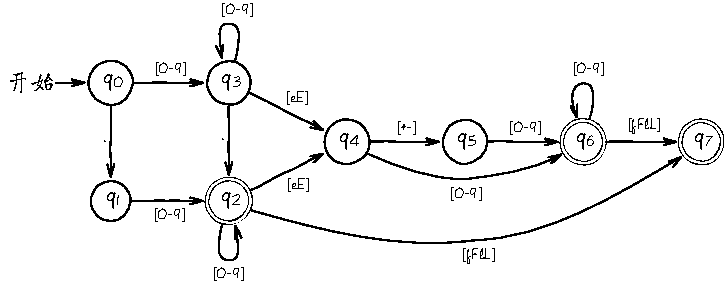
\includegraphics[scale=1.5]{automata_hand.pdf}
  \caption{严教授手画的有限自动机:它描述了 C 语言中浮点型字面值的词法。}
  \label{fig:automatahand}
\end{figure}

然而,尽管\autoref{fig:automatahand} 中严教授的自动机画得很仔细,但要在他的课
程幻灯片中使用,还是太粗疏了。严教授需要的是色彩鲜明、清晰准确的自动机图形,
就像\autoref{fig:automata} 中的一样。
\begin{figure}[htpb]
  \centering
  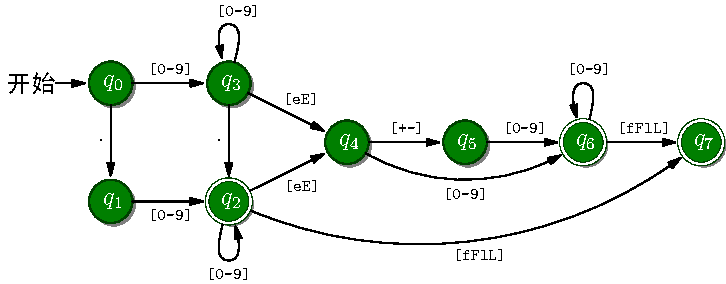
\includegraphics[scale=1.5]{automata.pdf}
  \caption{严教授想要在幻灯片里使用的有限自动机}
  \label{fig:automata}
\end{figure}

经过考虑,严教授决定用 \Asy{} 语言来完成这样的绘图,因为这样可以画出最精确的
图形,并能方便地对图形的所有细节进行控制,并且适合绘制大量形式相近的图形。然
而要让图形和生成图形的代码都接近完美,也将是一个艰巨的任务。

\section{标签和连线}
\label{sec:object}

把一些相似的小图形用线和箭头连接起来,是应用中非常广泛的一种作图类型。工作程
序的流程图、电路设计图、网络结构图、计算机科学中的自动机、乃至古老的家谱,都
可以看作是这类图形。这些相似的小图形往往是以一个文字标签为中心、用某种形状的
曲线围成的,再以各种线连接为一个整体——它可以抽象为数学中的“图”。这类图形
可以统称为图论图形,这正是计算机科学中使用最多的一类图形,也是严宇教授工作的
重点。

\Asy{} 语言已经提供了一种给标签围上边框,再连上线条的方法。这依赖于一种特殊的
数据类型:|object|(物件)。\index{object@\asyinline=object=}一个物件就是一个
带有某种形状边框的文字标签。函数
\index{draw@\asyinline=draw=}
\begin{asycode}
object draw(picture pic=currentpicture, Label L, envelope e,
            pair position=(0,0), real xmargin=0, real ymargin=xmargin,
            pen p=currentpen, filltype filltype=NoFill);
\end{asycode}
将在图 |pic| 上的位置 |position| 画出一个以标签 |L| 为中心,边框形状为 |e| 的
物件。参数 |xmargin| 和 |ymargin| 是边框与标签边沿的距离,画笔 |p| 用来绘制文
字标签,而 |filltype| 控制边框如何绘制和填充。
\index{filltype@\asyinline=filltype=}

\Asy{} 的这个函数初看起来非常复杂,但排除默认的参数,使用起来是直接了当的:
\begin{asycode}
object cat = draw("cat", box, (0,0), filltype=Draw),
       dog = draw("dog", ellipse, (2cm,0), filltype=Fill(olive)),
       elephant = draw("elephant", roundbox, (0,-2cm),
                       filltype=FillDraw(lightblue, darkblue));
\end{asycode}
\begin{figure}[H]
  \centering
\begin{asy}
object cat = draw("cat", box, (0,0), filltype=Draw),
       dog = draw("dog", ellipse, (2cm,0), filltype=Fill(olive)),
       elephant = draw("elephant", roundbox, (0,-2cm),
                       filltype=FillDraw(lightblue, darkblue));
\end{asy}
\end{figure}
\index{box@\asyinline=box=} \index{ellipse@\asyinline=ellipse=}
\index{roundbox@\asyinline=roundbox=} \index{Draw@\asyinline=Draw=}
\index{Fill@\asyinline=Fill=} \index{FillDraw@\asyinline=FillDraw=}
这里 |box|、|ellipse| 和 |roundbox| 分别是矩形、椭圆和圆角矩形三种可以使用的
形状;|Draw|、|Fill|、|FillDraw| 则分别是对边框画线、填充的控制变量(参考
\cite{asyman})。调用 |draw| 函数时如果省略 |filltype| 参数,则这里的默认值
|NoFill| 效果和 |Draw| 一样,表示使用画笔 |p| 绘制边框。

下面的问题则是把这些物件用线连接起来。为此,\Asy{} 提供了一种看起来颇为古怪的
方式:
\begin{asycode}
add(
    new void(picture pic, transform t) {
        draw(pic, point(cat,E,t) -- point(dog,W,t), Arrow);
        draw(pic, point(cat,S,t) -- point(elephant,N,t), Arrow);
        draw(pic, point(elephant,NE,t) -- point(dog,SW,t), Arrows);
        draw(pic, "curve", point(cat,SW,t) {SW} .. {SE} point(elephant,NW,t));
    }
);
\end{asycode}
\begin{figure}[H]
  \centering
\begin{asy}
object cat = draw("cat", box, (0,0), filltype=Draw),
       dog = draw("dog", ellipse, (2cm,0), filltype=Fill(olive)),
       elephant = draw("elephant", roundbox, (0,-2cm),
                       filltype=FillDraw(lightblue, darkblue));
add(
    new void(picture pic, transform t) {
        draw(pic, point(cat,E,t) -- point(dog,W,t), Arrow);
        draw(pic, point(cat,S,t) -- point(elephant,N,t), Arrow);
        draw(pic, point(elephant,NE,t) -- point(dog,SW,t), Arrows);
        draw(pic, "curve", point(cat,SW,t) {SW} .. {SE} point(elephant,NW,t));
    }
);
\end{asy}
\end{figure}
\index{add@\asyinline=add=}
在这里,实际只有一条语句 |add|,但 |add| 的参数则是一个匿名函数:
\index{函数!匿名函数}
\begin{asycode}
new void (picture pic, trasform t) {
    // `\color{comment}匿名函数体`
}
\end{asycode}
意思是在 |currentpicture|(|add| 省略的第一个参数)实际进行绘图时,就使用这个
匿名函数中的语句进行绘图\footnote{这种用法并没有在手册 \cite{asyman} 中描述,
它涉及 \asyinline=picture= 图类型内部的实现方式。这里添加的匿名函数就相当于添
加了一个等效的 \asyinline=drawer= 类型的函数。参看
\prgname{plain\_picture.asy} 中的代码。}。

上面匿名函数的内容就是画出 |cat|、|dog|、|elephant| 之间的连线,其中用到了有
关 |object| 物件类型的一个函数 |point|\footnote{函数 \asyinline=point= 也没有
在手册 \cite{asyman} 中描述。关于此函数以及预置的物件形状 \asyinline=box=、
\asyinline=roundbox= 和 \asyinline=ellipse= 的定义,参看
\prgname{plain\_boxes.asy} 中的代码。}:
\index{point@\asyinline=point=}
\begin{asycode}
pair point(object F, pair dir, transform t=identity());
\end{asycode}
这个函数输出物件 |F| 的边框在 |dir| 方向的坐标。这个坐标通过 |t| 作变换。注意
这里的方向 |dir| 是经过边框形状矫正过的,因而对于矩形物件,|NE| 方向的坐标点
就是矩形右上方向的直角点,而并非严格的 $45^\circ$ 角方向点。在匿名函数中,必
须把匿名函数的参数 |t| 传给函数 |point|,并且绘图时在参数 |pic| 的图中进行,
才能保证在正确的位置以正确的比例画出物件的坐标和连线。

在匿名函数中,只要注意正确地使用 |point| 函数和 |t|、|pic| 参数,对于绘图的语
句没有特别的限制。因此上面无论是连直线、曲线、箭头还是在连线上标注文字,都和
普通的方式一样。

尽管语法多少有些难看和冗繁,但使用 \Asy{} 中的物件类型和它的连线机制,就足够
画出各种形式的图论图形了。严教授的自动机也可以这样逐步构造出来。然而,严教授
最终却放弃了这种绘图的方式。不是因为这种方式的写法麻烦,而是因为这种方式很难
表达出一些有用的功能。例如,仅指定物件而不使用 |point| 函数指定具体连线的位置
来连接两个物件的能力,如在下面的代码中,我们能不能不去手工指定 |cat| 和 |dog|
的方向 |ENE| 和 |WSW| 呢?
\begin{asycode}
object cat = draw("cat", box, (0,0), filltype=Draw),
       dog = draw("dog", ellipse, (3cm,2cm), filltype=Fill(olive));
add(
    new void(picture pic, transform t) {
        draw(point(cat,ENE,t) -- point(dog,WSW,t));
    }
);
\end{asycode}
\begin{figure}[H]
  \centering
\begin{asy}
object cat = draw("cat", box, (0,0), filltype=Draw),
       dog = draw("dog", ellipse, (3cm,2cm), filltype=Fill(olive));
add(
    new void(picture pic, transform t) {
        draw(point(cat,ENE,t) -- point(dog,WSW,t));
    }
);
\end{asy}
\end{figure}
确实,如果是复杂的图论图形,靠人力算出连点合适的方向来,一不留神就会出错;而
如果想要通过一个循环自动化地连接五角星形呢?
\begin{figure}[H]
  \centering
\begin{asy}
import "figure-src/node.asy" as node;
real u = 1.5cm;
node[] p;
for (int i = 0; i < 5; ++i) {
    p[i] = Circle(string(i+1), u*dir(90+72i), drawer);
    draw(p[i]);
}
p.cyclic = true;
for (int i = 0; i < 5; ++i) {
    draw(p[i] -- p[i+2], Arrow);
    draw(p[i] .. bendright .. p[i+1], Arrow);
}
\end{asy}
\end{figure}
想要利用现有的 |object| 类型的连线机制画出上面的图形无疑就太麻烦了,因为定义
分布在正五边形上的五个物件或进行连线并不难(参看第\ref{chap:stars}章五角星的
画法),但要精确地确定五个圆形上连线的位置就非常令人头疼了。而严教授更希望他
能以一种更简单更自然的方式画连线,比如说:
\begin{asycode}
draw(cat -- dog);
\end{asycode}
如果真的可以这样做连线的话,那么要画出前面的五角星形就容易得多了。

不仅如此,还有一些工作是超出目前的 |object| 类型能力的。例如,产生 |object|
的 |draw| 函数只能支持 |box|、|ellipse| 和 |roundbox| 三种形状,而使用的
|filltype| 参数也只有 |FillDraw|、|Fill|、|Draw|、|NoFill|、|UnFill|、
|RadialShade|(参看 \cite{asyman})这么有限的几种。如果我们想要画出图形:
\begin{figure}[H]
  \centering
\begin{asy}
import "figure-src/node.asy" as node;
draw(Circle("A", (0,0), compose(shadow,filldrawer(yellow))));
draw(Circle("B", (2cm,0), white, ballshade));
\end{asy}
\end{figure}
那么我们就要增加新的圆形,新的带阴影的和带球形立体效果的 |filltype|——但在仔
细研究 \Asy{} 本身实现 |filltype| 和 |object| 相关类型的代码之前,我们甚至不
知道这种扩充能不能做到。在这种情况下,或者是通过研读 \Asy{} 中
\prgname{plain} 等基本模块(\Asy{} 在安装时就预定义好了许多模块,而其中最基本
的 \prgname{plain} 模块则会在运行时自动导入,我们平时使用的 \Asy{} 实际是建立
在 \prgname{plain} 模块之上的)的代码,自行扩充;或者需要自己重新实现一个新类
型。实际中很难说哪种方式更简单或更好用,但研究 \Asy{} 中 \prgname{plain} 模块
的实现,总是有教益的。

\section[解析代码与扩充功能]{解析代码与扩充功能\footnote{本节一些内容不易理解
,初次阅读时可跳过。}}
\label{sec:analyzecode}

下面我们就考虑上一节最后提出的一个简单问题:增加新的圆形 |envelope|。为此,我
们需要分析 \Asy{} 中 \prgname{plain} 模块的部分实现,然后对它进行扩充和修改。

在 \prgname{plain} 模块的一个子模块 \prgname{plain\_boxes.asy} 中,定义了有关
生成 |object| 类型的 |draw| 函数和 |box|、|roundbox|、|ellipse| 三种
|envelope| 类型的形状,|point| 函数的定义也在其中。如果我们需要新定义一种圆形
形状 |circle|,就可以模仿里面的代码。在研究相关的代码时,可能需要不断查阅手册
\cite{asyman}。

首先在 \prgname{plain\_boxes.asy} 的中间可以找到 |evelope| 类型的定义:
\index{envelope@\asyinline=envelope=}
\begin{asycode}
typedef path envelope(frame dest, frame src=dest, real xmargin=0,
                      real ymargin=xmargin, pen p=currentpen,
                      filltype filltype=NoFill, bool above=true);
\end{asycode}
这里使用了 |typedef| 命令定义类型的别名。\index{typedef@\asyinline=typedef=}
|typedef| 命令的用法是
\begin{asycode}
typedef `对标识符 foo 的声明`;
\end{asycode}
表示把 |foo| 定义为它所声明的类型的一个别名。如
\begin{asycode}
typedef int Integer;
\end{asycode}
就把 |Integer| 定义为整数类型 |int| 的别名,从而以后就可以用 |Integer| 来代替
|int|。上面就把 |envelope| 定义为一个函数类型的别名\footnote{但在 \Asy{} 中,
函数类型的别名只能用来声明一个函数变量,不能用于定义一个有函数体的函数。},这
个函数接受许多参数,而返回一条路径。不难猜想,这个函数返回的路径,正是将来生
成 |object| 类型元素的形状。

此时再看 \prgname{plain\_boxes.asy} 开头,就看到了 |box|、|roundbox| 和
|ellipse| 的定义,实际就是定义了三个函数。例如 |ellipse| 的定义(这里的代码来
自 \Asy{} 1.90 版本):
\begin{asycode}[numbers=left]
path ellipse(frame dest, frame src=dest, real xmargin=0, real ymargin=xmargin,
             pen p=currentpen, filltype filltype=NoFill, bool above=true)
{
  pair m=min(src);
  pair M=max(src);
  pair D=M-m;
  static real factor=0.5*sqrt(2);
  int sign=filltype == NoFill ? 1 : -1;
  path g=ellipse(0.5*(M+m),factor*D.x+0.5*sign*max(p).x+xmargin,
                 factor*D.y+0.5*sign*max(p).y+ymargin);
  frame F;
  if(above == false) {
    filltype.fill(F,g,p);
    prepend(dest,F);
  } else filltype.fill(dest,g,p);
  return g;
\end{asycode}
这个函数初看起来可能有点复杂。但如果只看它的返回值的话,那么函数主要的工作就
是返回路径 |g|,也就是 9、10 两行定义的椭圆。现在来分析函数的其他部分,4、5 
行定义的坐标 |m| 和 |M| 就是帧 |src| 的左下角和右下角点。其中帧\index{帧}
|frame|\index{frame@\asyinline=frame=} 是 \Asy{} 中类似于图 |picture| 的一种
功能更简单更基本的类型,不支持诸如自动放缩的功能;而函数
|min|\index{min@\asyinline=min=} 和 |max|\index{max@\asyinline=max=} 则接受帧
、图、路径甚至画笔(表示笔尖的路径)作为参数,分别返回它们的左下角和右上角的
坐标。于是,第 6 行定义的坐标 |D| 就是帧 |src| 的对角线向量。第 7 行定义了一
个静态(|static|\footnote{ 在这里表示一个常量,用静态类型保证只进行一次赋值。
有关静态类型请参看手册 \cite{asyman}。}\index{静态}
\index{static@\asyinline=static=})的实数因子 |factor| 为 $\sqrt{2}/2$。第 8
行判断填充类型 |filltype| 是否为空的 |NoFill| 而设置一个符号 |sign|。这样,9
、10 两行定义的椭圆就清楚了,它的中心就是帧 |src| 的中心,坐标为 $(M+m)/2$;
它的横轴半径是因子 |factor| 乘以对角线向量的横坐标 |D.x|,加上(或当
|filltype| 不为 |NoFill| 时减去)笔尖边框右上角位置的横坐标的一半\footnote{不
难发现其实这个实现是错误的,原来的代码试图给长轴加上笔尖宽度的一半,以保证即
使画笔很粗,也可以让边框线与标签内容间有正确的距离;由于笔尖的路径相对于原点
对称,这里计算笔尖边框右上角坐标的一半,其实只是笔尖宽度的 $1/4$。正确的实现
应该是 \asyinline{0.5*sign*(max(p)-min(p))}。在 1.91 以后版本的 \Asy{} 中,这
个错误已经修正。},
再加上用户定义的距离 |xmargin|;纵轴的定义与长轴类似。后面的 11
至 15 行,实际就是根据 |above| 的具体取值,对边框的填充和画线(|above| 为假时
在目标帧 |dest| 底部绘制)。

通过对比不难发现,|box| 与 |roundbox| 的实现与 |ellipse| 实际上大同小异。因此
我们很容易模仿它们写出圆形的 |envelope| 函数\footnote{修正了椭圆中计算轴长方
法中的小错误。}:
\begin{asycode}
// `\color{comment}circle 函数就是一个 envelope 类型的变量`
path circle(frame dest, frame src=dest, real xmargin=0, real ymargin=xmargin,
             pen p=currentpen, filltype filltype=NoFill, bool above=true)
{
    pair m=min(src);
    pair M=max(src);
    pair D=M-m;
    static real factor=0.5*sqrt(2);
    int sign=filltype == NoFill ? 1 : -1;
    // `\color{comment}圆的半径 r 就是前面定义中椭圆的横轴与纵轴中的较大值`
    real r = max(factor*D.x+sign*max(p).x+xmargin,
                 factor*D.y+sign*max(p).y+ymargin);
    path g=circle(0.5*(M+m), r);
    frame F;
    if(above == false) {
        filltype.fill(F,g,p);
        prepend(dest,F);
    } else filltype.fill(dest,g,p);
    return g;
}
\end{asycode}

把这段代码放在前面,马上就可以试验效果:
\begin{asycode}
object cat = draw("cat", circle, (0,0)),
       dog = draw("dog", circle, (2cm,0), filltype=Fill(olive));
add(
    new void(picture pic, transform t) {
        draw(point(cat,E,t) -- point(dog,W,t), Arrow);
    }
);
\end{asycode}
\begin{figure}[H]
  \centering
\begin{asy}
path circle(frame dest, frame src=dest, real xmargin=0, real ymargin=xmargin,
             pen p=currentpen, filltype filltype=NoFill, bool above=true)
{
    pair m=min(src);
    pair M=max(src);
    pair D=M-m;
    static real factor=0.5*sqrt(2);
    int sign=filltype == NoFill ? 1 : -1;
    real r = max(factor*D.x+sign*max(p).x+xmargin,
                 factor*D.y+sign*max(p).y+ymargin);
    path g=circle(0.5*(M+m), r);
    frame F;
    if(above == false) {
        filltype.fill(F,g,p);
        prepend(dest,F);
    } else filltype.fill(dest,g,p);
    return g;
}

object cat = draw("cat", circle, (0,0)),
       dog = draw("dog", circle, (2cm,0), filltype=Fill(olive));
add(
    new void(picture pic, transform t) {
        draw(point(cat,E,t) -- point(dog,W,t), Arrow);
    }
);
\end{asy}
\end{figure}

这样,通过分析并模仿 \prgname{plain} 模块原有的代码,就完成了一种新的
|envelope| 形状 |circle|,并能将其付诸使用。

但是,有关 |envelope| 类型的函数是比较复杂的,要想真正看懂它,像上面这样分析
清楚,甚至可能需要了解一些手册 \cite{asyman} 中没有提及的东西,也就是分析更多
的源代码。例如上面 |filltype| 的内部结构在手册中并没有给出说明,而需要分析
\prgname{plain\_filldraw.asy} 的代码;以画笔为参数的函数 |max| 也没有文档,更
需要到 \Asy{} 的 C++ 代码 \prgname{runtime.in} 和 \prgname{pen.h} 中才能找到
定义。

上面分析 |ellipse| 函数的过程可以看做一般的分析 \Asy{} 源代码的一个缩影。有时
所分析的代码比较简单,可以像上面那样比较容易地看清楚代码的来龙去脉,并对它进
行必要的扩充和修改;有时问题则会变得困难,需要缺少文档的情况下,在许多个源文
件中搜索需要的定义(比如由 |ellipse| 的定义查找 |filltype| 的内部结构和 |max|
函数在 \prgname{runtime.in} 中的定义)。并非人人像严教授这样是这方面的专家,
在很多情况下,分析源代码耗费的精力会比重写一遍相同功能的代码还要多,甚至会遇
到看不懂源代码的情形。这时,就必须要考虑解决问题的其他途径了。

\section{结构体与抽象机制}
\label{sec:struct}

出于对功能的扩充和最终用法简洁性的要求,严教授还是决定自己来设计一个新的类型
来完成他的自动机的绘制。

\Asy{} 中的数据类型是十分丰富的,除了整数(|int|)、实数(|real|)、坐标(
|pair|,即复数)、路向(|guide|)、路径(|path|)等基本类型,还有画笔(|pen|
)、图(|picture|)等预置的复杂类型,还有函数和数组类型。然而,更重要的是,
\Asy{} 还有把这些类型组合起来,建立新类型的一般方法,也就是对数据的抽象机制,
这就是结构体。\Asy{} 中的结构体与 C/C++ 语言的结构体在语法上十分接近,同时也
有自己的特点。\index{结构体}

一个结构体类型用下面的语法定义:
\index{struct@\asyinline=struct=}
\begin{asycode}
struct `结构体名` {
    `类型$_1$` `成员变量$_1$`;
    `类型$_2$` `成员变量$_2$`;
    `……`
}
\end{asycode}
这样,就把若干个类型的变量结合为一个整体,形成一个新的类型。例如,可以把两个
实数类型的变量复合为一种新的坐标类型:
\begin{asycode}
struct newpair {
    real x, y;
}
\end{asycode}
于是,就可以使用这种新的类型 |newpair| 来声明一个复合类型的变量,并且像普通
的 |pair| 类型一样,可以使用圆点运算符来分别得到它的两个分量:
\begin{asycode}
newpair a;     // `\color{comment}定义 newpair 类型的变量 a`
a.x = 1.0;      // `\color{comment}给 a 的 x 分量赋值`
a.y = 2.5;      // `\color{comment}给 a 的 y 分量赋值`
\end{asycode}
这样,就可以用一个变量名 |a| 表示相互紧密联系的两个量 |a.x| 和 |a.y|。这就是
数据的抽象。

物件类型 |object| 实际上就是把一个表示边框的路径和边框中的内容结合组成的结构
体\footnote{参看 \prgname{plain\_Label.asy} 的源代码。}。严教授需要的也就是与
|object| 类型的一个类似的类型,使用相同的方法,把一个边框路径、它的内容(用图
表示)以及它的位置结合为一个结构,并命名为“结点”|node|:
\begin{asycode}
// `\color{comment}结点类型,第一个实现`
struct node {
    path outline;   // `\color{comment}边框`
    picture stuff;  // `\color{comment}内容`
    pair pos;       // `\color{comment}位置`
}
\end{asycode}
于是,就可以写出这样的语句:
\begin{asycode}
node cat;                                   // `\color{comment}定义 cat 结点`
cat.outline = circle((0,0), 4mm);           // `\color{comment}cat 的边框是一个圆`
cat.pos = (0,0);                            // `\color{comment}cat 的位置在原点`
filldraw(cat.stuff, cat.outline, yellow);   // `\color{comment}把边框画进 cat 的内容`
label(cat.stuff, "cat");                    // `\color{comment}把文字标进 cat 的内容`
add(shift(cat.pos) * cat.stuff);            // `\color{comment}在指定位置画出 cat 的内容`
\end{asycode}
\begin{figure}[H]
  \centering
\begin{asy}
struct node {
    path outline;
    picture stuff;
    pair pos;
}
node cat;
label(cat.stuff, "cat");
cat.outline = circle((0,0), 4mm);
cat.pos = (0,0);
filldraw(cat.stuff, cat.outline, yellow);
add(cat.stuff);
\end{asy}
\end{figure}
这无疑是十分简陋的,还远远比不上 |object| 类型的精致。但这已经展示出了操作
|node| 类型的最重要的手段。下面要做的事就是,用函数把上面的一个个独立的操作包
装起来。

首先是使用函数建立一个 |node| 类型的变量,它的内容是一个文字标签,边框是紧密
围绕在标签之外的一个圆形,而位置由函数的参数指定。不仅如此,还要指定边框和标
签分别怎么在 |node| 的内容中画出来,最简单的办法就是分别指定一些画笔:
\begin{asycode}
// `\color{comment}圆形结点的构造函数,第一个实现`
node Circle(Label text, pair pos, pen textpen=currentpen,
            pen fillpen=nullpen, pen drawpen=currentpen)
{
    node nd;        // `\color{comment}定义新结点`
    nd.pos = pos;   // `\color{comment}设置位置`
    label(nd.stuff, text, textpen);             // `\color{comment}在内容中标注文字`
    pair M = max(nd.stuff), m = min(nd.stuff);  // `\color{comment}计算内容边界大小`
    nd.outline = circle(0.5*(M+m), 0.5*length(M-m));    // `\color{comment}设置边框`
    filldraw(nd.stuff, nd.outline, fillpen, drawpen);   // `\color{comment}绘制和填充边框`
    return nd;      // `\color{comment}返回构造的新结点`
}
\end{asycode}
这里计算内容边界并设置圆形边框路径的办法,就是前面为 |object| 类型建立圆形
|envelope| 的算法的特别简化的版本:计算出左下、右上角的坐标,得到中心坐标和对
角线长度,就是边框的圆心和直径。

然后是定义一个函数画出整个结点,方法和单独把结点的内容加进当前图一样:
\begin{asycode}
// `\color{comment}画结点,简单实现`
void draw(picture pic=currentpicture, node nd)
{
    add(pic, shift(nd.pos) * nd.stuff);
}
\end{asycode}

于是,利用上面的函数,就可以这样来画出结点了:
\begin{asycode}
node cat = Circle("cat", (0,0), fillpen=yellow),
     dog = Circle("dog", (2cm,0), fillpen=olive, drawpen=nullpen);
draw(cat);
draw(dog);
\end{asycode}
\begin{figure}[H]
  \centering
\begin{asy}
struct node {
    path outline;
    picture stuff;
    pair pos;
}
node Circle(Label text, pair pos, pen textpen=currentpen,
            pen fillpen=nullpen, pen drawpen=currentpen)
{
    node nd;
    nd.pos = pos;
    label(nd.stuff, text, textpen);
    pair M = max(nd.stuff), m = min(nd.stuff);
    nd.outline = circle(0.5*(M+m), 0.5*length(M-m));
    filldraw(nd.stuff, nd.outline, fillpen, drawpen);
    return nd;
}
void draw(picture pic=currentpicture, node nd)
{
    add(pic, shift(nd.pos) * nd.stuff);
}
node cat = Circle("cat", (0,0), fillpen=yellow),
     dog = Circle("dog", (2cm,0), fillpen=olive, drawpen=nullpen);
draw(cat);
draw(dog);
\end{asy}
\end{figure}

现在来看怎么实现 |object| 类型中 |point| 函数的对应物。类似 |point(cat,E,t)|
的用法无疑是太蹩脚了,比如理想的方式是 |cat.E|。按前面 |node| 类型的定义,只
要给 |node| 增加一组变量,分别保存边框在不同方向上的点的坐标。但更一般地,直
接得到边框在某个特定方向(或角度)上的点也是非常有用的,因此最好还有一种类似
|point.angle(30)| 或 |point.dir(ENE)| 的语法,来表示边框上的特定方向的点。对
此,也只要在结构体 |node| 中增加几个函数类型作为成员。因此,可以这样扩充
|node| 类型:
\begin{asycode}
// `\color{comment}结点类型,第二个实现`
struct node {
    path outline;
    picture stuff;
    pair pos;
    pair E, N, W, S;
    pair dir(pair v)
    {
        path g = shift(pos) * outline;
        pair M = max(g), m = min(g), c = 0.5*(M+m);
        path ray = c -- c + length(M-m)*unit(v);
        return intersectionpoint(g, ray);
    }
    pair angle(real ang)
    {
        return this.dir(dir(ang));
    }
}
\end{asycode}

这里需要解释的函数是新加进来的 |dir| 函数。就像上面做的,在结构体中可以直接定
义函数,即这个结构体的成员函数\index{成员函数}\index{结构体!成员函数}。在
\Asy{} 中,成员函数也是结构体的普通成员变量,结构体里面的函数定义只是给了这个
变量一个初始值。在 |dir| 函数中,它接受一个表示方向的坐标变量 |v|,返回从结点
边框的中心发出的在 |v| 方向的射线与边框路径的交点,也就是我们要的边框在 |v| 
方向上的点。|dir| 函数的计算过程是简单而清晰的:首先通过平移得到正确的边框路
径 |g|,而后计算边框的右上角坐标 |M|、左下角坐标 |m|、中心坐标 |c|,而后计算
射线 |ray|,最后返回交点坐标。其中用到的 |length|
\index{length@\asyinline=length=} 函数计算向量的长度(也就是对应复数的绝对值
),|unit|\index{unit@\asyinline=unit=} 函数计算与向量方向相同的单位向量,而
|intersectionpoint| 正是 \autoref{sec:guide2path} 中的求两路径交点的函数。在
成员函数 |dir| 中,可以直接使用结构体里面定义的变量,而不必再通过参数传递,这
正是结构体成员函数的方便之处。

另一个成员函数 |angle| 只是简单地调用刚刚定义的 |dir| 函数,完成类似的功能。
不过这里的语句有点令人疑惑:前面对 |dir| 的定义实际是重载了 \Asy{} 本来就有一
个函数 |dir|,因而 |angle| 要使用两个 |dir| 函数,一个是成员函数 |dir(pair)| 
计算交点,另一个是系统的 |dir(real)| 计算一个角度方向上的向量。正像前面
\autoref{sec:randomarray} 中所说的,重载的两个函数参数类型不同,所以可以直接
用 |dir(dir(ang))|,并不会产生歧义,但为了避免读代码的人混淆,这里用了
|this.dir| 来表示结构体的成员函数。|this|\index{this@\asyinline=this=} 是一个
特殊的关键字,可以用来代替这个结构体类型的实例本身(如已经定义了 |node| 类型
的变量 |a|,那么调用 |a.angle(0)| 时,|a.angle| 函数中的 |this| 就代表 |a| 本
身,从而 |this.dir| 就是 |a.dir|)。

此时,结点类型 |node| 增加了 |E|、|N|、|W|、|S| 几个坐标用来方便地访问边框上
的点,这些坐标也必须在用函数构造结点类型时就进行初始化。这就需要在 |Circle| 
函数中增加几个语句,调用成员函数 |dir| 函数完成这个工作:
\begin{asycode}
// `\color{comment}圆形结点的构造函数,第二个实现`
node Circle(Label text, pair pos, pen textpen=currentpen,
            pen fillpen=nullpen, pen drawpen=currentpen)
{
    node nd;
    nd.pos = pos;
    label(nd.stuff, text, textpen);
    pair M = max(nd.stuff), m = min(nd.stuff);
    nd.outline = circle(0.5*(M+m), 0.5*length(M-m));
    filldraw(nd.stuff, nd.outline, fillpen, drawpen);
    nd.E = nd.dir(E);   // `\color{comment}调用 nd.dir 函数对四个方向初始化`
    nd.N = nd.dir(N);
    nd.W = nd.dir(W);
    nd.S = nd.dir(S);
    return nd;
}
\end{asycode}

对结点类型的 |draw| 函数不需要做改变。因此,下面就不仅可以画出结点,而且可以
像使用原来的 |object| 类型一样,画出连线了:
\begin{asycode}
node cat = Circle("cat", (0,0), fillpen=yellow),
     dog = Circle("dog", (2cm,0), fillpen=olive, drawpen=nullpen);
draw(cat);
draw(dog);
draw(cat.E -- dog.W, Arrow);
// `\color{comment}等价地,也可以用`
// draw(cat.dir(E) -- cat.dir(W), Arrow);
// `\color{comment}或者`
// draw(cat.angle(0) -- cat.angle(180), Arrow);
\end{asycode}
\begin{figure}[H]
  \centering
\begin{asy}
// `\color{comment}结点类型,第二个实现`
struct node {
    path outline;
    picture stuff;
    pair pos;
    pair E, N, W, S;
    pair dir(pair v)
    {
        path g = shift(pos) * outline;
        pair M = max(g), m = min(g), c = 0.5*(M+m);
        path ray = c -- c + length(M-m)*unit(v);
        return intersectionpoint(g, ray);
    }
    pair angle(real ang)
    {
        return this.dir(dir(ang));
    }
}

// `\color{comment}圆形结点的构造函数,第二个实现`
node Circle(Label text, pair pos, pen textpen=currentpen,
            pen fillpen=nullpen, pen drawpen=currentpen)
{
    node nd;
    nd.pos = pos;
    label(nd.stuff, text, textpen);
    pair M = max(nd.stuff), m = min(nd.stuff);
    nd.outline = circle(0.5*(M+m), 0.5*length(M-m));
    filldraw(nd.stuff, nd.outline, fillpen, drawpen);
    nd.E = nd.dir(E);
    nd.N = nd.dir(N);
    nd.W = nd.dir(W);
    nd.S = nd.dir(S);
    return nd;
}

void draw(picture pic=currentpicture, node nd)
{
    add(pic, shift(nd.pos) * nd.stuff);
}

node cat = Circle("cat", (0,0), fillpen=yellow),
     dog = Circle("dog", (2cm,0), fillpen=olive, drawpen=nullpen);
draw(cat);
draw(dog);
draw(cat.E -- dog.W, Arrow);
// `\color{comment}等价地,也可以用`
// draw(cat.dir(E) -- cat.dir(W), Arrow);
// `\color{comment}或者`
// draw(cat.angle(0) -- cat.angle(180), Arrow);
\end{asy}
\end{figure}

现在,利用结构体进行数据抽象,定义函数对抽象数据类型进行操作,我们就已经完成
了对原来 \Asy{} 中预定义的 |object| 类型一个简单的模拟。在这个过程中,我们失
去了一些功能:新的 |node| 类型不能使用 |size| 函数正确地进行放缩,因为它并不
像 |object| 类型在绘制时还小心冀冀地处理一个变换 |t|(见
\autoref{sec:object});也没有像原来的 |object| 类型那样在计算边框线粗细等细
节上锱铢必较(见 \autoref{sec:analyzecode})。但也得到了许多好处,那就是使用
时的简洁、清晰和容易修改扩充。而要完成这些,只要二三十行的代码。对比代码
\begin{asycode}
draw(cat.E -- dog.W);
\end{asycode}
和
\begin{asycode}
add(
    new void(picture pic, transform t) {
        draw(point(cat,E,t) -- point(cat,W,t));
    }
;)
\end{asycode}
其实不难做出抉择。

\section{运算符和记法}
\label{sec:operator}

然而,严教授并不满足于让 |node| 重复 |object| 类型的功能,他需要的是更简单、
更有效的写法:
\begin{asycode}
draw(cat -- dog);
\end{asycode}
尽管看上去差别不大,但从 |cat.E| 到 |cat| 的转变是本质性的,这个区别比从
|point(cat,E,t)| 到 |cat.E| 的区别还要大。因为无论是 |point(cat,E,t)| 还是
|cat.E|,都是一个 |pair| 类型的量,用它来连线是顺理成章的;但 |cat| 则是
|node| 类型的变量,两个 |node| 类型的变量用 |--| 连起来是什么东西?它们又怎么
能连起来呢?

这就引发了一个新的问题,就是发明一种把两个 |node| 类型连接起来的新的记法。而
这个语法是本来在 \Asy{} 中是没有的。要完成这一点,就需要使用运算符的重载。
\index{运算符重载}\index{重载!运算符重载}

在 \Asy{} 中,像 |+|、|-|、|*|、|/| 以及 |--|、|..| 这些运算符,都可以看成是
一个以 |operator|\index{operator@\asyinline=operator=} 开头的函数
\footnote{在 \Asy{} 中,绝大部分运算符都可以看做是函数,从而可以重载,甚至包
括一些在基本语言中没有的运算符,如 \asyinline=@=。但也有一些例外,包括赋值、
圆点、中括号(下标)、圆括号(函数调用)和条件运算符。}。如整数的加法运算符
|+| 就等价于函数
\begin{asycode}
int operator+(int op1, int op2);
\end{asycode}
它接受两个整数参数,返回它们的和。因而 |1+2| 就等价于 |operator+(1,2)|,都得
到结果 |3|。

既然运算符就是函数,那么就可以自己定义;即使已经有了定义,按照
\autoref{sec:randomarray} 中所说,也可以自己重载。因而,完全可以通过重载,定
义一种不寻常的整数加法:
\begin{asycode}
// `\color{comment}保存旧的加法定义`
int oldadd(int op1, int op2) = operator+;
// `\color{comment}定义新的加法为模 5 意义下的加法`
int operator+(int op1, int op2)
{
    return oldadd(op1, op2) % 5;
}
\end{asycode}
也就是把加号 |+| 定义为 $\mathbb{Z}_5$ 上的加法运算了。那么 |1+2| 的结果仍然
是 |3|,但 |2+3| 的结果就成了 |0|,|2+4| 则得到 |1|。

这样,利用自定义运算符 |--|,严教授就顺理成章地完成了两个结点之间的连线定义:
\begin{asycode}
path operator--(node nd1, node nd2)
{
    path g1 = shift(nd1.pos) * nd1.outline;
    path g2 = shift(nd2.pos) * nd2.outline;
    pair c1 = (max(g1)+min(g1)) / 2;
    pair c2 = (max(g2)+min(g2)) / 2;
    path edge = c1 -- c2;
    edge = firstcut(edge, g1).after;
    edge = lastcut(edge, g2).before;
    return edge;
}
\end{asycode}
这里,|operator--| 函数接受两个结点参数。它首先计算两个结点的边框路径 |g1| 和
|g2|,然后算出两个边框的中心 |c1| 和 |c2|,然后定义结点的连线 |edge| 就是
|c1 -- c2|,最后利用 |firstcut| 和 |lastcut| 函数截取 |edge| 在 |g1| 交点后面
、在 |g2| 交点前面的中间一段,就是正确的连线。
\index{firstcut@\asyinline=firstcut=}
\index{lastcut@\asyinline=lastcut=}

在这里,函数 |firstcut| 和 |lastcut| 分别是函数 |cut|
\index{cut@\asyinline=cut=} 的在 |n| 为 |0| 和 |-1| 时的特例:
\begin{asycode}
slice cut(path p, path knife, int n);
\end{asycode}
|cut| 函数返回一个结构体 |slice|\index{slice@\asyinline=slice=}:
\index{before@\asyinline=before=}
\index{after@\asyinline=after=}
\begin{asycode}
struct slice {
    path before,after;
}
\end{asycode}
它计算路径 |p| 与 |knife| 的第 |n| 个(负数表示倒数)交点,把 |p| 分成两半:
其中 |before| 是把路径 |p| 用“刀” |knife| 切开的前半截,而 |after| 是后半截
。

好了,现在严教授就可以这样画出两个结点及连线了:
\begin{asycode}
node cat = Circle("cat", (0,0), fillpen=yellow),
     dog = Circle("dog", (2cm,0), fillpen=olive, drawpen=nullpen);
draw(cat);
draw(dog);
draw(cat -- dog, Arrow);
\end{asycode}
\begin{figure}[H]
  \centering
\begin{asy}
// `\color{comment}结点类型,第二个实现`
struct node {
    path outline;
    picture stuff;
    pair pos;
    pair E, N, W, S;
    pair dir(pair v)
    {
        path g = shift(pos) * outline;
        pair M = max(g), m = min(g), c = 0.5*(M+m);
        path ray = c -- c + length(M-m)*unit(v);
        return intersectionpoint(g, ray);
    }
    pair angle(real ang)
    {
        return this.dir(dir(ang));
    }
}

// `\color{comment}圆形结点的构造函数,第二个实现`
node Circle(Label text, pair pos, pen textpen=currentpen,
            pen fillpen=nullpen, pen drawpen=currentpen)
{
    node nd;
    nd.pos = pos;
    label(nd.stuff, text, textpen);
    pair M = max(nd.stuff), m = min(nd.stuff);
    nd.outline = circle(0.5*(M+m), 0.5*length(M-m));
    filldraw(nd.stuff, nd.outline, fillpen, drawpen);
    nd.E = nd.dir(E);
    nd.N = nd.dir(N);
    nd.W = nd.dir(W);
    nd.S = nd.dir(S);
    return nd;
}

void draw(picture pic=currentpicture, node nd)
{
    add(pic, shift(nd.pos) * nd.stuff);
}

path operator--(node nd1, node nd2)
{
    path g1 = shift(nd1.pos) * nd1.outline;
    path g2 = shift(nd2.pos) * nd2.outline;
    pair c1 = (max(g1)+min(g1)) / 2;
    pair c2 = (max(g2)+min(g2)) / 2;
    path edge = c1 -- c2;
    edge = firstcut(edge, g1).after;
    edge = lastcut(edge, g2).before;
    return edge;
}

node cat = Circle("cat", (0,0), fillpen=yellow),
     dog = Circle("dog", (2cm,0), fillpen=olive, drawpen=nullpen);
draw(cat);
draw(dog);
draw(cat -- dog, Arrow);
\end{asy}
\end{figure}

事情还没有完。上面只是定义了两个结点之间的直线连接,严教授还需要用曲线把结点
连接起来。也就是说,严教授还希望有某种方便的 |..| 运算符。

理想中的 |..| 运算符应该是什么样的?回想第\ref{chap:tiling}章中曲线的绘制。把
两个结点直接用 |..| 连起来是没有什么用的,因为 |cat..dog| 就应该得到一条直线
,那么 |cat--dog| 就足够了;而 |cat{NE}..{SE}dog| 这种记法合理一些,但也好不
到哪里去,因为它并不比 |cat.dir(NE){NE}..{SE}dog.dir(SW)| 简单多少,同样需要
手工去设想准确的连接方向。至于 |tension|、|curl| 等,更难看出实际的用处来。
——说到底,严教授需要的是一种完全不同于以往的记法。考虑这个图形:
\begin{asycode}
node cat = Circle("cat", (0,0), fillpen=yellow),
     dog = Circle("dog", (5cm,0), fillpen=olive, drawpen=nullpen);
draw(cat);
draw(dog);
draw(cat.angle(30){dir(30)} .. {dir(-30)}dog.angle(150), Arrow);
\end{asycode}
\begin{figure}[H]
  \centering
\begin{asy}
// `\color{comment}结点类型,第二个实现`
struct node {
    path outline;
    picture stuff;
    pair pos;
    pair E, N, W, S;
    pair dir(pair v)
    {
        path g = shift(pos) * outline;
        pair M = max(g), m = min(g), c = 0.5*(M+m);
        path ray = c -- c + length(M-m)*unit(v);
        return intersectionpoint(g, ray);
    }
    pair angle(real ang)
    {
        return this.dir(dir(ang));
    }
}

// `\color{comment}圆形结点的构造函数,第二个实现`
node Circle(Label text, pair pos, pen textpen=currentpen,
            pen fillpen=nullpen, pen drawpen=currentpen)
{
    node nd;
    nd.pos = pos;
    label(nd.stuff, text, textpen);
    pair M = max(nd.stuff), m = min(nd.stuff);
    nd.outline = circle(0.5*(M+m), 0.5*length(M-m));
    filldraw(nd.stuff, nd.outline, fillpen, drawpen);
    nd.E = nd.dir(E);
    nd.N = nd.dir(N);
    nd.W = nd.dir(W);
    nd.S = nd.dir(S);
    return nd;
}

void draw(picture pic=currentpicture, node nd)
{
    add(pic, shift(nd.pos) * nd.stuff);
}

path operator--(node nd1, node nd2)
{
    path g1 = shift(nd1.pos) * nd1.outline;
    path g2 = shift(nd2.pos) * nd2.outline;
    pair c1 = (max(g1)+min(g1)) / 2;
    pair c2 = (max(g2)+min(g2)) / 2;
    path edge = c1 -- c2;
    edge = firstcut(edge, g1).after;
    edge = lastcut(edge, g2).before;
    return edge;
}

node cat = Circle("cat", (0,0), fillpen=yellow),
     dog = Circle("dog", (5cm,0), fillpen=olive, drawpen=nullpen);
draw(cat);
draw(dog);
draw(cat.angle(30){dir(30)} .. {dir(-30)}dog.angle(150), Arrow);
\end{asy}
\end{figure}
最后一行的曲线连线看起来十分复杂,出现了四个角度,但它们其实加起来只表示一个
意思:就是从 |cat| 从左边偏 $30^\circ$ 连一条曲线拐到 |dog|,这个 $30^\circ$
是相对 |cat| 和 |dog| 的直线连线而说的。因此,看起来合情合理的记法就呼之欲出
了,它可以是这个样子的:
\begin{asycode}
draw(cat .. bendleft .. dog, Arrow);
\end{asycode}
这个记法很像是定义路向控制点的 |z0 .. controls c .. z1| 记法,因而也很容易理
解。而前面利用 |angle| 成员函数对 |cat| 和 |dog| 连线的复杂的写法,实际上揭示
了这个记法的实现方法。

如果不考虑新记法的问题,首先可以实现把两个结点用曲线连起来的一个函数。不妨就
叫它 |bendleft|:
\begin{asycode}
// `\color{comment}用弯曲路径连接两个结点,第一个实现`
path bendleft(node nd1, node nd2)
{
    path g1 = shift(nd1.pos) * nd1.outline;
    path g2 = shift(nd2.pos) * nd2.outline;
    pair c1 = (max(g1)+min(g1)) / 2;
    pair c2 = (max(g2)+min(g2)) / 2;
    real deg = degrees(c2 - c1);
    return nd1.angle(deg+30) {dir(deg+30)}
        .. {dir(deg-30)} nd2.angle(180+deg-30);
}
\end{asycode}
前面的计算就和直线连接一样,找出了两个结点的中心坐标 |c1| 和 |c2|。最后利用
|degrees| 函数(它计算向量的角度,正是 |dir| 函数的反函数),计算了直线
|c1--c2| 的角度 |deg|。最后返回的曲线路径就和前面直接连接 |cat| 和 |dog| 的过
程差不多,只是考虑了 |deg| 的影响:所谓向左偏 $30^\circ$,其实就是在角度
|deg| 的基础上加上 $30^\circ$,从而得到 |nd1| 边框上点的角度和在这点的曲线切
线方向,类似地可以得到 |nd2| 相关的角度。

要得到 |nd1 .. bendleft .. nd2| 这种新的记法,那大概就应该是一个接受三个参数
的运算符函数:
\begingroup
\renewcommand\thelstnumber{?}
\begin{asycode}[numbers=left]
typedef path edgeconnector(node nd1, node nd2);

path operator..(node nd1, edgeconnector con, node nd2)
{
    return con(nd1, nd2);
}
\end{asycode}
\endgroup
这里利用 |typedef| 定义了一个连线的 |edgeconnector| 类型,其实就是从两个结点
连成一条路径的函数类型的别名。然后就让 |operator..| 函数接受两个结点和一个连
线函数,返回用这个函数计算得到的连线。

可惜,当我们用 |cat .. bendleft .. dog| 来测试这段代码的使用时,\Asy{} 毫不留
情地发出了一条错误信息:
\begin{asycode}
`no matching function` 'operator ..(node, path(node nd1, node nd2))'
\end{asycode}
分析这条错误信息我们发现,\Asy{} 并不把 |cat .. bendleft .. dog| 看成是一个整
体,而是先按从左到右的优先级,去计算 |cat .. bendleft|,然后发现没有这种运算
符的定义的错误。这无疑是说,想要用一个 |operator..| 函数授受三个不同的参数的
做法是成功不了的,前面的定义是错误的。

看上去问题陷入了僵局:我们已经定义了十分方便的 |cat -- dog|,却无法正确定义
|cat .. bendleft .. dog|,而不得不使用 |bendleft(cat, dog)|。后一种函数调用的
记法并不复杂,但缺乏一致性。

然而严教授总有办法:既然 \Asy{} 只允许 |cat .. bendleft|,那么何不就让它先算
出一个正确的 |cat .. bendleft| 呢?可以让 |cat .. bendleft| 先算出一个中间值
(比如说 |f|),它包含 |cat| 和 |bendleft| 的全部信息,然后再计算 |f .. dog|
以 |bendleft(cat,dog)| 作为结果。这个过程有点技巧性,关键是需要一个中间值,它
仍然得是一个新的类型。

有两种实现中间值的办法,一种是使用结构体,一种是建立一个一元函数。严教授选择
了后一种,因为它更简洁,也更能体现函数作为一种动态数据的作用:
\begin{asycode}
typedef path edgeconnector(node nd1, node nd2);
typedef path edgemaker(node nd);

// `\color{comment}nd1 .. con .. nd2 的前一半`
edgemaker operator..(node nd, edgeconnector con)
{
    return new path(node nd2) {
        return con(nd, nd2);
    };
}

// `\color{comment}nd1 .. con .. nd2 的后一半`
path operator..(edgemaker maker, node nd)
{
    return maker(nd);
}
\end{asycode}
这时,使用
\begin{asycode}
draw(cat .. bendleft .. dog, Arrow);
\end{asycode}
就能画出正确的图形了。注意,严教授在函数 |operator..(node,edgeconnector)| 中
直接返回了一个新的函数,也就是一个 |edgemaker| 的对象。
\index{函数!作为返回值}

类似地,还可以定义右弯的函数 |bendright|,这和 |bendleft| 函数的区别仅仅在于
$30^\circ$ 的符号。不过严教授使用了更一般的方式定义了一个向任意角度弯转的
|bend| 函数:
\begin{asycode}
// `\color{comment}用弯曲路径连接两个结点,第二个实现`
edgeconnector bend(real ang)
{
    return new path (node nd1, node nd2) {
        path g1 = shift(nd1.pos) * nd1.outline;
        path g2 = shift(nd2.pos) * nd2.outline;
        pair c1 = (max(g1)+min(g1)) / 2;
        pair c2 = (max(g2)+min(g2)) / 2;
        real deg = degrees(c2 - c1);
        return nd1.angle(deg+ang) {dir(deg+ang)}
            .. {dir(deg-ang)} nd2.angle(180+deg-ang);
    };
}

edgeconnector bendleft = bend(30);
edgeconnector bendright = bend(-30);
\end{asycode}
这里,|edgeconnector| 类型的函数被作为 |bend| 的返回值得到,因而 |bendleft| 
就被定义为 |bend(30)|,而 |bendright| 被定义为 |bend(-30)|。如果需要更多的东
西,甚至还可以加上构造曲线的 |tension| 值,扩充的余地还有很大。

更进一步,严教授还需要给他的自动机画循环的函数,来画出这样的图形来:
\begin{figure}[H]
  \centering
\begin{asy}
// `\color{comment}结点类型,第二个实现`
struct node {
    path outline;
    picture stuff;
    pair pos;
    pair E, N, W, S;
    pair dir(pair v)
    {
        path g = shift(pos) * outline;
        pair M = max(g), m = min(g), c = 0.5*(M+m);
        path ray = c -- c + length(M-m)*unit(v);
        return intersectionpoint(g, ray);
    }
    pair angle(real ang)
    {
        return this.dir(dir(ang));
    }
}

// `\color{comment}圆形结点的构造函数,第二个实现`
node Circle(Label text, pair pos, pen textpen=currentpen,
            pen fillpen=nullpen, pen drawpen=currentpen)
{
    node nd;
    nd.pos = pos;
    label(nd.stuff, text, textpen);
    pair M = max(nd.stuff), m = min(nd.stuff);
    nd.outline = circle(0.5*(M+m), 0.5*length(M-m));
    filldraw(nd.stuff, nd.outline, fillpen, drawpen);
    nd.E = nd.dir(E);
    nd.N = nd.dir(N);
    nd.W = nd.dir(W);
    nd.S = nd.dir(S);
    return nd;
}

void draw(picture pic=currentpicture, node nd)
{
    add(pic, shift(nd.pos) * nd.stuff);
}

path operator--(node nd1, node nd2)
{
    path g1 = shift(nd1.pos) * nd1.outline;
    path g2 = shift(nd2.pos) * nd2.outline;
    pair c1 = (max(g1)+min(g1)) / 2;
    pair c2 = (max(g2)+min(g2)) / 2;
    path edge = c1 -- c2;
    edge = firstcut(edge, g1).after;
    edge = lastcut(edge, g2).before;
    return edge;
}

typedef path edgeconnector(node nd1, node nd2);
typedef path edgemaker(node nd);

// `\color{comment}nd1 .. con .. nd2 的前一半`
edgemaker operator..(node nd, edgeconnector con)
{
    return new path(node nd2) {
        return con(nd, nd2);
    };
}

// `\color{comment}nd1 .. con .. nd2 的后一半`
path operator..(edgemaker maker, node nd)
{
    return maker(nd);
}

edgeconnector bend(real ang)
{
    return new path (node nd1, node nd2) {
        path g1 = shift(nd1.pos) * nd1.outline;
        path g2 = shift(nd2.pos) * nd2.outline;
        pair c1 = (max(g1)+min(g1)) / 2;
        pair c2 = (max(g2)+min(g2)) / 2;
        real deg = degrees(c2 - c1);
        return nd1.angle(deg+ang) {dir(deg+ang)}
            .. {dir(deg-ang)} nd2.angle(180+deg-ang);
    };
}

edgeconnector bendleft = bend(30);
edgeconnector bendright = bend(-30);

path operator..(node nd, edgemaker maker)
{
    return maker(nd);
}

// `\color{comment}自动机循环`
edgemaker loop(pair direction, real ratio=1.5)
{
    return new path(node nd) {
        real deg = degrees(direction);
        real angle1 = deg - 15, angle2 = deg + 15;
        pair mid = nd.angle(deg)
            + ratio*fontsize(currentpen)*unit(direction);
        return nd.angle(angle1) {dir(angle1)} .. mid
            .. {-dir(angle2)} nd.angle(angle2);
    };
}

node cat = Circle("cat", (0,0), fillpen=yellow);
draw(cat);
draw(cat .. loop(up), Arrow);
\end{asy}
\end{figure}
现在只要对 |cat| 一个结点向自己做连线,怎样的记法才是最自然的呢?直接用函数的
形式 |loop(cat)| 就不错,如果需要确定循环连线的方向,那么 |loop(cat,up)| 也不
错。不过严教授坚持在连线时使用统一的记法,那么比较好的写法就应该是
\begin{asycode}
draw(cat .. loop(up), Arrow);
\end{asycode}

有了前面的东西,这个循环的记法并不难实现。而且严教授在前面定义的 |edgemaker|
类型在这里得到了应用:
\begin{asycode}
path operator..(node nd, edgemaker maker)
{
    return maker(nd);
}

// `\color{comment}自动机循环`
edgemaker loop(pair direction, real ratio=1.5)
{
    return new path(node nd) {
        real deg = degrees(direction);
        real angle1 = deg - 15, angle2 = deg + 15;
        pair mid = nd.angle(deg)
            + ratio*fontsize(currentpen)*unit(direction);
        return nd.angle(angle1) {dir(angle1)} .. mid
            .. {-dir(angle2)} nd.angle(angle2);
    };
}
\end{asycode}

最后,严教授发现,像 \autoref{sec:struct} 中那样每画一个结点就用一个 |draw| 
函数的方法也不是什么好的记法。理想的办法应该是可以在一个 |draw| 函数中使用任
意多个结点,就像
\begin{asycode}
draw(cat, dog, elephant);
\end{asycode}
这种方式。然而,要使用“任意多个”参数,就必须依赖 \Asy{} 的一种新的语法了,
那就是可变长参数表。

\index{可变长参数}\index{函数!可变长参数}
带有可变长参数的函数原型为:
\begin{asycode}
`返回类型` function(`前面的参数` ... T[] `数组`)
\end{asycode}
其中使用 |...| 把前面的参数和最后的一个数组类型的参数分开(中间没有逗号),前
面的参数和普通的函数参数一样,最后一个数组由在函数参数列表的末尾所有类型为
|T| 的那些参数构成。因为这些参数放在函数参数表的最后,所以在 \Asy{} 中又被称
为剩余参数(rest arguments)。\index{剩余参数}\index{函数!剩余参数}

因而,如果画出一个结点数组的函数是
\begin{asycode}
// `\color{comment}画出结点数组`
void draw(picture pic=currentpicture, node[] nodearr)
{
    for (node nd: nodearr)
        add(pic, shift(nd.pos) * nd.stuff);
}
\end{asycode}
则画出一次多个结点的函数就是
\begin{asycode}
// `\color{comment}画出一个或多个结点`
void draw(picture pic=currentpicture ... node[] nodearr)
{
    draw(pic, nodearr);
}
\end{asycode}
在 |draw| 的代码中,严教授又使用了一种新的 |for| 循环记法:
\index{for@\asyinline=for=}
\begin{asycode}
for (elem : arr)
    `循环语句体`
\end{asycode}
表示让 |elem| 取遍数组 |arr| 中的元素进行循环。

最终,把所有这些东西都用在一起,就足够用相当简洁的语法画出一个完整的自动机的
图形了(\autoref{fig:automatapreliminary}):
\begin{asycode}
real u = 2cm;
pen StateText = white;
pen StateFill = deepgreen;
pen StateDraw = darkgreen+0.6;
pen AcceptDraw = darkgreen+1.8;
node q0 = Circle("$q_0$", (0,0), StateText, StateFill, StateDraw),
     q1 = Circle("$q_1$", q0.pos + u*S, StateText, StateFill, StateDraw),
     q2 = Circle("$q_2$", q1.pos + u*E, StateText, StateFill, AcceptDraw),
     q3 = Circle("$q_3$", q0.pos + u*E, StateText, StateFill, StateDraw),
     q4 = Circle("$q_4$", q3.pos + u*E + 0.5u*S, StateText, StateFill, StateDraw),
     q5 = Circle("$q_5$", q4.pos + u*E, StateText, StateFill, StateDraw),
     q6 = Circle("$q_6$", q5.pos + u*E, StateText, StateFill, AcceptDraw),
     q7 = Circle("$q_7$", q6.pos + u*E, StateText, StateFill, AcceptDraw);
draw(q0, q1, q2, q3, q4, q5, q6, q7);
pen edgepen = fontcommand("\scriptsize\ttfamily");
draw(".",     q0 -- q1, edgepen, Arrow);
draw("[0-9]", q1 -- q2, edgepen, Arrow);
draw(".",     q3 -- q2, edgepen, Arrow);
draw("[eE]",  q2 -- q4, edgepen, Arrow);
draw(Label("[0-9]", LeftSide),  q0 -- q3, edgepen, Arrow);
draw(Label("[eE]", LeftSide),   q3 -- q4, edgepen, Arrow);
draw(Label("[+-]", LeftSide),   q4 -- q5, edgepen, Arrow);
draw(Label("[0-9]", LeftSide),  q5 -- q6, edgepen, Arrow);
draw(Label("[fFlL]", LeftSide), q6 -- q7, edgepen, Arrow);
draw("[0-9]", q3 .. loop(N), edgepen, Arrow);
draw("[0-9]", q2 .. loop(S), edgepen, Arrow);
draw("[0-9]", q6 .. loop(N), edgepen, Arrow);
draw("[0-9]",  q4 .. bendright .. q6, edgepen, Arrow);
draw("[fFlL]", q2 .. bendright .. q7, edgepen, Arrow);
\end{asycode}
\begin{figure}[htbp]
  \centering
\begin{asy}
// `\color{comment}结点类型,第二个实现`
struct node {
    path outline;
    picture stuff;
    pair pos;
    pair E, N, W, S;
    pair dir(pair v)
    {
        path g = shift(pos) * outline;
        pair M = max(g), m = min(g), c = 0.5*(M+m);
        path ray = c -- c + length(M-m)*unit(v);
        return intersectionpoint(g, ray);
    }
    pair angle(real ang)
    {
        return this.dir(dir(ang));
    }
}

// `\color{comment}圆形结点的构造函数,第二个实现`
node Circle(Label text, pair pos, pen textpen=currentpen,
            pen fillpen=nullpen, pen drawpen=currentpen)
{
    node nd;
    nd.pos = pos;
    label(nd.stuff, text, textpen);
    pair M = max(nd.stuff), m = min(nd.stuff);
    nd.outline = circle(0.5*(M+m), 0.5*length(M-m));
    filldraw(nd.stuff, nd.outline, fillpen, drawpen);
    nd.E = nd.dir(E);
    nd.N = nd.dir(N);
    nd.W = nd.dir(W);
    nd.S = nd.dir(S);
    return nd;
}

// `\color{comment}画出结点数组`
void draw(picture pic=currentpicture, node[] nodearr)
{
    for (node nd: nodearr)
        add(pic, shift(nd.pos) * nd.stuff);
}

// `\color{comment}画出一个或多个结点`
void draw(picture pic=currentpicture ... node[] nodearr)
{
    draw(pic, nodearr);
}

path operator--(node nd1, node nd2)
{
    path g1 = shift(nd1.pos) * nd1.outline;
    path g2 = shift(nd2.pos) * nd2.outline;
    pair c1 = (max(g1)+min(g1)) / 2;
    pair c2 = (max(g2)+min(g2)) / 2;
    path edge = c1 -- c2;
    edge = firstcut(edge, g1).after;
    edge = lastcut(edge, g2).before;
    return edge;
}

typedef path edgeconnector(node nd1, node nd2);
typedef path edgemaker(node nd);

// `\color{comment}nd1 .. con .. nd2 的前一半`
edgemaker operator..(node nd, edgeconnector con)
{
    return new path(node nd2) {
        return con(nd, nd2);
    };
}

// `\color{comment}nd1 .. con .. nd2 的后一半`
path operator..(edgemaker maker, node nd)
{
    return maker(nd);
}

edgeconnector bend(real ang)
{
    return new path (node nd1, node nd2) {
        path g1 = shift(nd1.pos) * nd1.outline;
        path g2 = shift(nd2.pos) * nd2.outline;
        pair c1 = (max(g1)+min(g1)) / 2;
        pair c2 = (max(g2)+min(g2)) / 2;
        real deg = degrees(c2 - c1);
        return nd1.angle(deg+ang) {dir(deg+ang)}
            .. {dir(deg-ang)} nd2.angle(180+deg-ang);
    };
}

edgeconnector bendleft = bend(30);
edgeconnector bendright = bend(-30);

path operator..(node nd, edgemaker maker)
{
    return maker(nd);
}

// `\color{comment}自动机循环`
edgemaker loop(pair direction, real ratio=1.5)
{
    return new path(node nd) {
        real deg = degrees(direction);
        real angle1 = deg - 15, angle2 = deg + 15;
        pair mid = nd.angle(deg)
            + ratio*fontsize(currentpen)*unit(direction);
        return nd.angle(angle1) {dir(angle1)} .. mid
            .. {-dir(angle2)} nd.angle(angle2);
    };
}

real u = 2cm;
pen StateText = white;
pen StateFill = deepgreen;
pen StateDraw = darkgreen+0.6;
pen AcceptDraw = darkgreen+1.8;
node q0 = Circle("$q_0$", (0,0), StateText, StateFill, StateDraw),
     q1 = Circle("$q_1$", q0.pos + u*S, StateText, StateFill, StateDraw),
     q2 = Circle("$q_2$", q1.pos + u*E, StateText, StateFill, AcceptDraw),
     q3 = Circle("$q_3$", q0.pos + u*E, StateText, StateFill, StateDraw),
     q4 = Circle("$q_4$", q3.pos + u*E + 0.5u*S, StateText, StateFill, StateDraw),
     q5 = Circle("$q_5$", q4.pos + u*E, StateText, StateFill, StateDraw),
     q6 = Circle("$q_6$", q5.pos + u*E, StateText, StateFill, AcceptDraw),
     q7 = Circle("$q_7$", q6.pos + u*E, StateText, StateFill, AcceptDraw);
draw(q0, q1, q2, q3, q4, q5, q6, q7);
pen edgepen = fontcommand("\scriptsize\ttfamily");
draw(".",     q0 -- q1, edgepen, Arrow);
draw("[0-9]", q1 -- q2, edgepen, Arrow);
draw(".",     q3 -- q2, edgepen, Arrow);
draw("[eE]",  q2 -- q4, edgepen, Arrow);
draw(Label("[0-9]", LeftSide),  q0 -- q3, edgepen, Arrow);
draw(Label("[eE]", LeftSide),   q3 -- q4, edgepen, Arrow);
draw(Label("[+-]", LeftSide),   q4 -- q5, edgepen, Arrow);
draw(Label("[0-9]", LeftSide),  q5 -- q6, edgepen, Arrow);
draw(Label("[fFlL]", LeftSide), q6 -- q7, edgepen, Arrow);
draw("[0-9]", q3 .. loop(N), edgepen, Arrow);
draw("[0-9]", q2 .. loop(S), edgepen, Arrow);
draw("[0-9]", q6 .. loop(N), edgepen, Arrow);
draw("[0-9]",  q4 .. bendright .. q6, edgepen, Arrow);
draw("[fFlL]", q2 .. bendright .. q7, edgepen, Arrow);
\end{asy}
  \caption{严教授初步完成的有限自动机}
  \label{fig:automatapreliminary}
\end{figure}

\autoref{fig:automatapreliminary} 已经完成了整个有限自动机的整体框架,而且用
来画出它的代码相当清晰,没有再玩弄看不清意义的变换 |t|,也完全免除了逐个考虑
连线起末点的坐标方向。这正是新记法的威力。下面,严教授将逐步精化这个图形,按
照理想中的要求,完善整个图形的细节。


\section{完善图形细节}

仔细审视\autoref{fig:automatapreliminary} 的效果,严教授发现理想中的几点要求
还没有做到:一是对于表示接受状态的结点 $q_2$, $q_6$, $q_7$,应该使用双线画出
,而不是现在这样用一条粗线代替;二是为了最终效果的美观,结点应该加上灰色阴影
的修饰;三是箭头显得太大,而且应该在末端处缩短一点,不与所指向的结点相接才好
看。阴影效果只是为了修饰,但双线效果却是正确画出有限自动机图形所必需的特征,
因而前面画出的似是而非的图形是不能拿到讲台上的。此外,原来手稿中的“开始”还
没有画出来,它只是一个普通的文字标签,但又像图的结点一样有连线,一时还拿不准
如何处理。

对于双线,首先想到的解决方案是画一大一小两条线。看上去只要把边框路径相对中心
做一个小小的放缩:
\begin{asycode}
path outline = circle((0,0), 1cm);
draw(outline ^^ scale(0.9)*outline);
\end{asycode}
\begin{figure}[H]
  \centering
\begin{asy}
path outline = circle((0,0), 1cm);
draw(outline ^^ scale(0.9)*outline);
\end{asy}
\end{figure}
然而这样做会带来许多问题:一是当放缩中心不在原点时,要进行比简单放缩更复杂的
变换;二是放缩比例难以正确的确定;第三点是最主要的,就是当边框不再是前面定义
的圆形时,其实任何放缩比例都不能得到正确的双线——距离中心远的地方双线距离也
远,距离中心近的地方双线距离太近:
\begin{asycode}
path outline = box((-3cm,-1cm), (3cm,1cm));
draw(outline ^^ scale(0.9)*outline, linewidth(1));  
\end{asycode}
\begin{figure}[H]
  \centering
\begin{asy}
path outline = box((-3cm,-1cm), (3cm,1cm));
draw(outline ^^ scale(0.9)*outline, linewidth(1));
\end{asy}
\end{figure}

其实得到双线的合适办法画一粗一细两条线,粗的是线的颜色,细的则是背景色,粗线
的宽度正好是细线的 3 倍:
\begin{asycode}
path outline = box((-3cm,-1cm), (3cm,1cm));
draw(outline, black+3);
draw(outline, white+1);  
\end{asycode}
\begin{figure}[H]
  \centering
\begin{asy}
path outline = box((-3cm,-1cm), (3cm,1cm));
draw(outline, black+3);
draw(outline, white+1);
\end{asy}
\end{figure}

再来看阴影。双线的解决办法是画两遍,其实阴影也是一样。要得到阴影效果,只要在
原来图形的后面平移一小块位置用灰色再填充一遍:
\begin{asycode}
path outline = circle((0,0), 1cm);
fill(shift(5SE) * outline, gray);
fill(outline, deepgreen);
\end{asycode}
\begin{figure}[H]
  \centering
\begin{asy}
path outline = circle((0,0), 1cm);
fill(shift(5SE) * outline, gray);
fill(outline, deepgreen);
\end{asy}
\end{figure}
不要这里要注意,前面的图形必须填充上颜色或者用
|unfill|\index{unfill@\asyinline=unfill=} 挖掉边框内的部分,否则灰色的阴影就
露馅了。

综合来看,前两个问题其实是相同的:那就是结点的绘制不再能简单地用三个画笔(文
字、填充、边框)描述清楚,而需要双线、阴影等更复杂的效果。这提示严教授必须修
改结点构造时的绘制过程,也必须修改结点的构造函数。

要实现复杂的绘制过程,最有效的办法莫过于使用函数。用根据边框进行复杂画图的函
数代替原来的画笔,就可以得到新的结点构造函数。首先给这种函数类型定义一个新的
别名:
\begin{asycode}
typedef void draw_t(picture pic, path g);
\end{asycode}
于是圆形结点就变成:
\begin{asycode}
// `\color{comment}圆形结点的构造函数,第三个实现`
node Circle(Label text, pair pos, pen textpen=currentpen,
            draw_t drawfn)
{
    node nd;
    nd.pos = pos;
    label(nd.stuff, text, textpen);
    pair M = max(nd.stuff), m = min(nd.stuff);
    nd.outline = circle(0.5*(M+m), 0.5*length(M-m));
    drawfn(nd.stuff, nd.outline);
    nd.E = nd.dir(E);
    nd.N = nd.dir(N);
    nd.W = nd.dir(W);
    nd.S = nd.dir(S);
    return nd;
}
\end{asycode}
形式上的改动是微小的:第二个实现中函数原型的 |fillpen| 和 |drawpen| 参数都代
以函数参数 |drawfn|,而原来绘制的 |filldraw| 语句也换成了 |drawfn| 语句。

不过这样一来,暂时就要使用这样的语句来构造结点了:
\begin{asycode}
node cat = Circle("cat", (0,0),
                  new void(picture pic, path g) {
                      filldraw(pic, g, yellow, black);
                  }
                 );
\end{asycode}
为了能让使用普通方法画结点还像原来一样方便,就得定义一些与 |fill|、|draw|、
|filldraw| 等对应的 |draw_t| 类型的函数:
\begin{asycode}
// `\color{comment}空函数,不做边框的绘制`
draw_t none = new void(picture pic, path g){};
// `\color{comment}画边框线`
draw_t drawer(pen p)
{
    return new void(picture pic, path g) {
        draw(pic, g, p);
    };
}
draw_t drawer=drawer(currentpen);
// `\color{comment}填充边框`
draw_t filler(pen p)
{
    return new void(picture pic, path g) {
        fill(pic, g, p);
    };
}
draw_t filler=filler(currentpen);
// `\color{comment}对边框填充并画线`
draw_t filldrawer(pen fillpen, pen drawpen=currentpen)
{
    return new void(picture pic, path g) {
        filldraw(pic, g, fillpen, drawpen);
    };
}
\end{asycode}
这里,|drawer(pen)| 函数返回一个用给定画笔画边框线的 |draw_t| 函数,但严教授
同时又定义 |drawer| 本身也是一个 |draw_t| 函数,使用当前画笔画线。类似地,填
充的 |filler| 也有两种形式。这实际上是利用了 \Asy{} 的函数重载功能(两个
|drawer|、两个 |filler| 其实都是参数不同的函数类型)。

于是,现在又可以像原来一样方便地画结点了:
\begin{asycode}
node cat = Circle("cat", (0,0), filldrawer(yellow, black)),
     dog = Circle("dog", (2cm,0), drawer);  //`\color{comment}drawer 相当于 drawer(currentpen)`
draw(cat, dog);
\end{asycode}
\begin{figure}[H]
  \centering
\begin{asy}
// `\color{comment}结点类型,第二个实现`
struct node {
    path outline;
    picture stuff;
    pair pos;
    pair E, N, W, S;
    pair dir(pair v)
    {
        path g = shift(pos) * outline;
        pair M = max(g), m = min(g), c = 0.5*(M+m);
        path ray = c -- c + length(M-m)*unit(v);
        return intersectionpoint(g, ray);
    }
    pair angle(real ang)
    {
        return this.dir(dir(ang));
    }
}

typedef void draw_t(picture pic, path g);

// `\color{comment}空函数,不做边框的绘制`
draw_t none = new void(picture pic, path g){};
// `\color{comment}画边框线`
draw_t drawer(pen p)
{
    return new void(picture pic, path g) {
        draw(pic, g, p);
    };
}
draw_t drawer=drawer(currentpen);
// `\color{comment}填充边框`
draw_t filler(pen p)
{
    return new void(picture pic, path g) {
        fill(pic, g, p);
    };
}
draw_t filler=filler(currentpen);
// `\color{comment}对边框填充并画线`
draw_t filldrawer(pen fillpen, pen drawpen=currentpen)
{
    return new void(picture pic, path g) {
        filldraw(pic, g, fillpen, drawpen);
    };
}


// `\color{comment}圆形结点的构造函数,第三个实现`
node Circle(Label text, pair pos, pen textpen=currentpen,
            draw_t drawfn)
{
    node nd;
    nd.pos = pos;
    label(nd.stuff, text, textpen);
    pair M = max(nd.stuff), m = min(nd.stuff);
    nd.outline = circle(0.5*(M+m), 0.5*length(M-m));
    drawfn(nd.stuff, nd.outline);
    nd.E = nd.dir(E);
    nd.N = nd.dir(N);
    nd.W = nd.dir(W);
    nd.S = nd.dir(S);
    return nd;
}

// `\color{comment}画出结点数组`
void draw(picture pic=currentpicture, node[] nodearr)
{
    for (node nd: nodearr)
        add(pic, shift(nd.pos) * nd.stuff);
}

// `\color{comment}画出一个或多个结点`
void draw(picture pic=currentpicture ... node[] nodearr)
{
    draw(pic, nodearr);
}

path operator--(node nd1, node nd2)
{
    path g1 = shift(nd1.pos) * nd1.outline;
    path g2 = shift(nd2.pos) * nd2.outline;
    pair c1 = (max(g1)+min(g1)) / 2;
    pair c2 = (max(g2)+min(g2)) / 2;
    path edge = c1 -- c2;
    edge = firstcut(edge, g1).after;
    edge = lastcut(edge, g2).before;
    return edge;
}

typedef path edgeconnector(node nd1, node nd2);
typedef path edgemaker(node nd);

// `\color{comment}nd1 .. con .. nd2 的前一半`
edgemaker operator..(node nd, edgeconnector con)
{
    return new path(node nd2) {
        return con(nd, nd2);
    };
}

// `\color{comment}nd1 .. con .. nd2 的后一半`
path operator..(edgemaker maker, node nd)
{
    return maker(nd);
}

edgeconnector bend(real ang)
{
    return new path (node nd1, node nd2) {
        path g1 = shift(nd1.pos) * nd1.outline;
        path g2 = shift(nd2.pos) * nd2.outline;
        pair c1 = (max(g1)+min(g1)) / 2;
        pair c2 = (max(g2)+min(g2)) / 2;
        real deg = degrees(c2 - c1);
        return nd1.angle(deg+ang) {dir(deg+ang)}
            .. {dir(deg-ang)} nd2.angle(180+deg-ang);
    };
}

edgeconnector bendleft = bend(30);
edgeconnector bendright = bend(-30);

path operator..(node nd, edgemaker maker)
{
    return maker(nd);
}

// `\color{comment}自动机循环`
edgemaker loop(pair direction, real ratio=1.5)
{
    return new path(node nd) {
        real deg = degrees(direction);
        real angle1 = deg - 15, angle2 = deg + 15;
        pair mid = nd.angle(deg)
            + ratio*fontsize(currentpen)*unit(direction);
        return nd.angle(angle1) {dir(angle1)} .. mid
            .. {-dir(angle2)} nd.angle(angle2);
    };
}

node cat = Circle("cat", (0,0), filldrawer(yellow, black)),
     dog = Circle("dog", (2cm,0), drawer);  //`\color{comment}drawer 相当于 drawer(currentpen)`
draw(cat, dog);
\end{asy}
\end{figure}

当然,问题的关键是完成画双线和阴影的复杂函数。有了前面的铺垫,画双线边框是轻
而易举的:
\begin{asycode}
// `\color{comment}画双线边框,第一个实现`
draw_t doubledrawer(pen p)
{
    return new void(picture pic, path g) {
        draw(pic, g, p+3*linewidth(p));
        draw(pic, g, white+linewidth(p));
    };
}
draw_t doubledrawer = doubledrawer(currentpen);

node cat = Circle("cat", (0,0), doubledrawer),
     dog = Circle("dog", (2cm,0), doubledrawer(red+1));
draw(cat, dog);
\end{asycode}
\begin{figure}[H]
  \centering
\begin{asy}
//#-*- coding: utf-8 -*-
// `\color{comment}结点类型,第二个实现`
struct node {
    path outline;
    picture stuff;
    pair pos;
    pair E, N, W, S;
    pair dir(pair v)
    {
        path g = shift(pos) * outline;
        pair M = max(g), m = min(g), c = 0.5*(M+m);
        path ray = c -- c + length(M-m)*unit(v);
        return intersectionpoint(g, ray);
    }
    pair angle(real ang)
    {
        return this.dir(dir(ang));
    }
}

typedef void draw_t(picture pic, path g);

// `\color{comment}空函数,不做边框的绘制`
draw_t none = new void(picture pic, path g){};
// `\color{comment}画边框线`
draw_t drawer(pen p)
{
    return new void(picture pic, path g) {
        draw(pic, g, p);
    };
}
draw_t drawer=drawer(currentpen);
// `\color{comment}填充边框`
draw_t filler(pen p)
{
    return new void(picture pic, path g) {
        fill(pic, g, p);
    };
}
draw_t filler=filler(currentpen);
// `\color{comment}对边框填充并画线`
draw_t filldrawer(pen fillpen, pen drawpen=currentpen)
{
    return new void(picture pic, path g) {
        filldraw(pic, g, fillpen, drawpen);
    };
}


// `\color{comment}圆形结点的构造函数,第三个实现`
node Circle(Label text, pair pos, pen textpen=currentpen,
            draw_t drawfn)
{
    node nd;
    nd.pos = pos;
    label(nd.stuff, text, textpen);
    pair M = max(nd.stuff), m = min(nd.stuff);
    nd.outline = circle(0.5*(M+m), 0.5*length(M-m));
    drawfn(nd.stuff, nd.outline);
    nd.E = nd.dir(E);
    nd.N = nd.dir(N);
    nd.W = nd.dir(W);
    nd.S = nd.dir(S);
    return nd;
}

// `\color{comment}画出结点数组`
void draw(picture pic=currentpicture, node[] nodearr)
{
    for (node nd: nodearr)
        add(pic, shift(nd.pos) * nd.stuff);
}

// `\color{comment}画出一个或多个结点`
void draw(picture pic=currentpicture ... node[] nodearr)
{
    draw(pic, nodearr);
}

path operator--(node nd1, node nd2)
{
    path g1 = shift(nd1.pos) * nd1.outline;
    path g2 = shift(nd2.pos) * nd2.outline;
    pair c1 = (max(g1)+min(g1)) / 2;
    pair c2 = (max(g2)+min(g2)) / 2;
    path edge = c1 -- c2;
    edge = firstcut(edge, g1).after;
    edge = lastcut(edge, g2).before;
    return edge;
}

typedef path edgeconnector(node nd1, node nd2);
typedef path edgemaker(node nd);

// `\color{comment}nd1 .. con .. nd2 的前一半`
edgemaker operator..(node nd, edgeconnector con)
{
    return new path(node nd2) {
        return con(nd, nd2);
    };
}

// `\color{comment}nd1 .. con .. nd2 的后一半`
path operator..(edgemaker maker, node nd)
{
    return maker(nd);
}

edgeconnector bend(real ang)
{
    return new path (node nd1, node nd2) {
        path g1 = shift(nd1.pos) * nd1.outline;
        path g2 = shift(nd2.pos) * nd2.outline;
        pair c1 = (max(g1)+min(g1)) / 2;
        pair c2 = (max(g2)+min(g2)) / 2;
        real deg = degrees(c2 - c1);
        return nd1.angle(deg+ang) {dir(deg+ang)}
            .. {dir(deg-ang)} nd2.angle(180+deg-ang);
    };
}

edgeconnector bendleft = bend(30);
edgeconnector bendright = bend(-30);

path operator..(node nd, edgemaker maker)
{
    return maker(nd);
}

// `\color{comment}自动机循环`
edgemaker loop(pair direction, real ratio=1.5)
{
    return new path(node nd) {
        real deg = degrees(direction);
        real angle1 = deg - 15, angle2 = deg + 15;
        pair mid = nd.angle(deg)
            + ratio*fontsize(currentpen)*unit(direction);
        return nd.angle(angle1) {dir(angle1)} .. mid
            .. {-dir(angle2)} nd.angle(angle2);
    };
}

// `\color{comment}画双线边框,第一个实现`
draw_t doubledrawer(pen p)
{
    return new void(picture pic, path g) {
        draw(pic, g, p+3*linewidth(p));
        draw(pic, g, white+linewidth(p));
    };
}
draw_t doubledrawer = doubledrawer(currentpen);

node cat = Circle("cat", (0,0), doubledrawer),
     dog = Circle("dog", (2cm,0), doubledrawer(red+1));
draw(cat, dog);
\end{asy}
\end{figure}
这个双线的实现考虑到了使用不同的边框画笔,并且自动计算画笔和白色背景的宽度,
看上去是完美无缺了。不过,严教授仍然不满意:这种实现方式还是不够一般,不仅背
景色不一定是白色的,而且结点可能不仅需要画双线,还需要填充、画阴影或是做别的
什么操作——有无数种组合的可能性,却必须为这每种可能性单独写一个 |draw_t| 类
型的函数。既然前面已经定义了画线、填充这些基本操作,那何不把它们组合起来呢?

严教授意识到,组合起多个 |draw_t| 函数,形成一个新的画结点边框的函数,这个功
能是的应用可能十分广泛。因此,他写出了把多个 |draw_t| 函数复合起来的函数,也
就是在复合函数中依次调用这些函数:
\begin{asycode}
// `\color{comment}多个边框绘制函数的复合`
draw_t compose(... draw_t[] drawfns)
{
    return new void(picture pic, path g) {
        for (draw_t f : drawfns)
            f(pic, g);
    };
}
\end{asycode}
这样,实现双线的函数就成为两个 |drawer| 的复合了:
\begin{asycode}
// `\color{comment}画双线边框,第二个实现`
draw_t doubledrawer(pen p, pen bg=white)
{
    return compose(drawer(p+linewidth(p)*3), drawer(bg+linewidth(p)));
}
draw_t doubledrawer = doubledrawer(currentpen);
\end{asycode}
更重要的是,可以更自由地组合不同的函数功能了:
\begin{asycode}
node cat = Circle("cat", (0,0), compose(filler(yellow), doubledrawer)),
     dog = Circle("dog", (2cm,0), compose(filler(olive), doubledrawer(darkgreen+1)));
draw(cat, dog);
\end{asycode}
\begin{figure}[H]
  \centering
\begin{asy}
// `\color{comment}结点类型,第二个实现`
struct node {
    path outline;
    picture stuff;
    pair pos;
    pair E, N, W, S;
    pair dir(pair v)
    {
        path g = shift(pos) * outline;
        pair M = max(g), m = min(g), c = 0.5*(M+m);
        path ray = c -- c + length(M-m)*unit(v);
        return intersectionpoint(g, ray);
    }
    pair angle(real ang)
    {
        return this.dir(dir(ang));
    }
}

// `\color{comment}边框绘制函数类型`
typedef void draw_t(picture pic, path g);

// `\color{comment}多个边框绘制函数的复合`
draw_t compose(... draw_t[] drawfns)
{
    return new void(picture pic, path g) {
        for (draw_t f : drawfns)
            f(pic, g);
    };
}

// `\color{comment}空函数,不做边框的绘制`
draw_t none = new void(picture pic, path g){};
// `\color{comment}画边框线`
draw_t drawer(pen p)
{
    return new void(picture pic, path g) {
        draw(pic, g, p);
    };
}
draw_t drawer=drawer(currentpen);
// `\color{comment}填充边框`
draw_t filler(pen p)
{
    return new void(picture pic, path g) {
        fill(pic, g, p);
    };
}
draw_t filler=filler(currentpen);
// `\color{comment}对边框填充并画线`
draw_t filldrawer(pen fillpen, pen drawpen=currentpen)
{
    return new void(picture pic, path g) {
        filldraw(pic, g, fillpen, drawpen);
    };
}


// `\color{comment}圆形结点的构造函数,第三个实现`
node Circle(Label text, pair pos, pen textpen=currentpen,
            draw_t drawfn)
{
    node nd;
    nd.pos = pos;
    label(nd.stuff, text, textpen);
    pair M = max(nd.stuff), m = min(nd.stuff);
    nd.outline = circle(0.5*(M+m), 0.5*length(M-m));
    drawfn(nd.stuff, nd.outline);
    nd.E = nd.dir(E);
    nd.N = nd.dir(N);
    nd.W = nd.dir(W);
    nd.S = nd.dir(S);
    return nd;
}

// `\color{comment}画出结点数组`
void draw(picture pic=currentpicture, node[] nodearr)
{
    for (node nd: nodearr)
        add(pic, shift(nd.pos) * nd.stuff);
}

// `\color{comment}画出一个或多个结点`
void draw(picture pic=currentpicture ... node[] nodearr)
{
    draw(pic, nodearr);
}

path operator--(node nd1, node nd2)
{
    path g1 = shift(nd1.pos) * nd1.outline;
    path g2 = shift(nd2.pos) * nd2.outline;
    pair c1 = (max(g1)+min(g1)) / 2;
    pair c2 = (max(g2)+min(g2)) / 2;
    path edge = c1 -- c2;
    edge = firstcut(edge, g1).after;
    edge = lastcut(edge, g2).before;
    return edge;
}

typedef path edgeconnector(node nd1, node nd2);
typedef path edgemaker(node nd);

// `\color{comment}nd1 .. con .. nd2 的前一半`
edgemaker operator..(node nd, edgeconnector con)
{
    return new path(node nd2) {
        return con(nd, nd2);
    };
}

// `\color{comment}nd1 .. con .. nd2 的后一半`
path operator..(edgemaker maker, node nd)
{
    return maker(nd);
}

edgeconnector bend(real ang)
{
    return new path (node nd1, node nd2) {
        path g1 = shift(nd1.pos) * nd1.outline;
        path g2 = shift(nd2.pos) * nd2.outline;
        pair c1 = (max(g1)+min(g1)) / 2;
        pair c2 = (max(g2)+min(g2)) / 2;
        real deg = degrees(c2 - c1);
        return nd1.angle(deg+ang) {dir(deg+ang)}
            .. {dir(deg-ang)} nd2.angle(180+deg-ang);
    };
}

edgeconnector bendleft = bend(30);
edgeconnector bendright = bend(-30);

path operator..(node nd, edgemaker maker)
{
    return maker(nd);
}

// `\color{comment}自动机循环`
edgemaker loop(pair direction, real ratio=1.5)
{
    return new path(node nd) {
        real deg = degrees(direction);
        real angle1 = deg - 15, angle2 = deg + 15;
        pair mid = nd.angle(deg)
            + ratio*fontsize(currentpen)*unit(direction);
        return nd.angle(angle1) {dir(angle1)} .. mid
            .. {-dir(angle2)} nd.angle(angle2);
    };
}

// `\color{comment}画双线边框,第二个实现`
draw_t doubledrawer(pen p, pen bg=white)
{
    return compose(drawer(p+linewidth(p)*3), drawer(bg+linewidth(p)));
}
draw_t doubledrawer = doubledrawer(currentpen);

node cat = Circle("cat", (0,0), compose(filler(yellow), doubledrawer)),
     dog = Circle("dog", (2cm,0), compose(filler(olive), doubledrawer(darkgreen+1)));
draw(cat, dog);
\end{asy}
\end{figure}

下面对于阴影,只要考虑阴影本身,阴影之外的功能都可以通过复合函数得到了。因而
画阴影的函数就很平常了:
\begin{asycode}
// `\color{comment}画阴影`
draw_t shadow(pair shift=2SE, real scale=1, pen color=gray)
{
    return new void(picture pic, path g) {
        fill(pic, shift(shift)*scale(scale)*g, color);
    };
}
draw_t shadow=shadow();
\end{asycode}
使用阴影时,因为阴影在图形的最下方,因而应该在复合函数的最前面:
\begin{asycode}
node cat = Circle("cat", (0,0), compose(shadow, filldrawer(yellow))),
     dog = Circle("dog", (2cm,0), compose(shadow, filler(olive)));
draw(cat, dog);
\end{asycode}
\begin{figure}[H]
  \centering
\begin{asy}
// `\color{comment}结点类型,第二个实现`
struct node {
    path outline;
    picture stuff;
    pair pos;
    pair E, N, W, S;
    pair dir(pair v)
    {
        path g = shift(pos) * outline;
        pair M = max(g), m = min(g), c = 0.5*(M+m);
        path ray = c -- c + length(M-m)*unit(v);
        return intersectionpoint(g, ray);
    }
    pair angle(real ang)
    {
        return this.dir(dir(ang));
    }
}

// `\color{comment}边框绘制函数类型`
typedef void draw_t(picture pic, path g);

// `\color{comment}多个边框绘制函数的复合`
draw_t compose(... draw_t[] drawfns)
{
    return new void(picture pic, path g) {
        for (draw_t f : drawfns)
            f(pic, g);
    };
}

// `\color{comment}空函数,不做边框的绘制`
draw_t none = new void(picture pic, path g){};
// `\color{comment}画边框线`
draw_t drawer(pen p)
{
    return new void(picture pic, path g) {
        draw(pic, g, p);
    };
}
draw_t drawer=drawer(currentpen);
// `\color{comment}填充边框`
draw_t filler(pen p)
{
    return new void(picture pic, path g) {
        fill(pic, g, p);
    };
}
draw_t filler=filler(currentpen);
// `\color{comment}对边框填充并画线`
draw_t filldrawer(pen fillpen, pen drawpen=currentpen)
{
    return new void(picture pic, path g) {
        filldraw(pic, g, fillpen, drawpen);
    };
}


// `\color{comment}圆形结点的构造函数,第三个实现`
node Circle(Label text, pair pos, pen textpen=currentpen,
            draw_t drawfn)
{
    node nd;
    nd.pos = pos;
    label(nd.stuff, text, textpen);
    pair M = max(nd.stuff), m = min(nd.stuff);
    nd.outline = circle(0.5*(M+m), 0.5*length(M-m));
    drawfn(nd.stuff, nd.outline);
    nd.E = nd.dir(E);
    nd.N = nd.dir(N);
    nd.W = nd.dir(W);
    nd.S = nd.dir(S);
    return nd;
}

// `\color{comment}画出结点数组`
void draw(picture pic=currentpicture, node[] nodearr)
{
    for (node nd: nodearr)
        add(pic, shift(nd.pos) * nd.stuff);
}

// `\color{comment}画出一个或多个结点`
void draw(picture pic=currentpicture ... node[] nodearr)
{
    draw(pic, nodearr);
}

path operator--(node nd1, node nd2)
{
    path g1 = shift(nd1.pos) * nd1.outline;
    path g2 = shift(nd2.pos) * nd2.outline;
    pair c1 = (max(g1)+min(g1)) / 2;
    pair c2 = (max(g2)+min(g2)) / 2;
    path edge = c1 -- c2;
    edge = firstcut(edge, g1).after;
    edge = lastcut(edge, g2).before;
    return edge;
}

typedef path edgeconnector(node nd1, node nd2);
typedef path edgemaker(node nd);

// `\color{comment}nd1 .. con .. nd2 的前一半`
edgemaker operator..(node nd, edgeconnector con)
{
    return new path(node nd2) {
        return con(nd, nd2);
    };
}

// `\color{comment}nd1 .. con .. nd2 的后一半`
path operator..(edgemaker maker, node nd)
{
    return maker(nd);
}

edgeconnector bend(real ang)
{
    return new path (node nd1, node nd2) {
        path g1 = shift(nd1.pos) * nd1.outline;
        path g2 = shift(nd2.pos) * nd2.outline;
        pair c1 = (max(g1)+min(g1)) / 2;
        pair c2 = (max(g2)+min(g2)) / 2;
        real deg = degrees(c2 - c1);
        return nd1.angle(deg+ang) {dir(deg+ang)}
            .. {dir(deg-ang)} nd2.angle(180+deg-ang);
    };
}

edgeconnector bendleft = bend(30);
edgeconnector bendright = bend(-30);

path operator..(node nd, edgemaker maker)
{
    return maker(nd);
}

// `\color{comment}自动机循环`
edgemaker loop(pair direction, real ratio=1.5)
{
    return new path(node nd) {
        real deg = degrees(direction);
        real angle1 = deg - 15, angle2 = deg + 15;
        pair mid = nd.angle(deg)
            + ratio*fontsize(currentpen)*unit(direction);
        return nd.angle(angle1) {dir(angle1)} .. mid
            .. {-dir(angle2)} nd.angle(angle2);
    };
}

// `\color{comment}画双线边框,第二个实现`
draw_t doubledrawer(pen p, pen bg=white)
{
    return compose(drawer(p+linewidth(p)*3), drawer(bg+linewidth(p)));
}
draw_t doubledrawer = doubledrawer(currentpen);

// `\color{comment}画阴影`
draw_t shadow(pair shift=2SE, real scale=1, pen color=gray)
{
    return new void(picture pic, path g) {
        fill(pic, shift(shift)*scale(scale)*g, color);
    };
}
draw_t shadow=shadow();

node cat = Circle("cat", (0,0), compose(shadow, filldrawer(yellow))),
     dog = Circle("dog", (2cm,0), compose(shadow, filler(olive)));
draw(cat, dog);
\end{asy}
\end{figure}

最后来看箭头的问题。在 \cite{asyman} 中,详细说明了箭头类型 |arrowhead| 的各
种参数,如使用 |Arrow(6)| 就表示使用 6\,bp 大小的箭头,修改也起来十分容易,例
如:
\begin{asycode}
Arrow = Arrow(6);
draw((0,0) -- (2cm,0), darkblue+2, Arrow);
\end{asycode}
\begin{figure}[H]
  \centering
\begin{asy}
Arrow = Arrow(6);
draw((0,0) -- (2cm,0), darkblue+2, Arrow);
\end{asy}
\end{figure}

然而要将箭头缩短一点,就没有现成的参数可用了。但可以把画箭头的曲线路径截短。
可以使用 \autoref{sec:guide2path} 中提及的
|subpath|\index{subpath@\asyinline=subpath=} 函数取路径的一段。于是只要知道所
截路径首尾的时间参数。严教授查了 \cite{asyman},得知可以使用
\index{arclength@\asyinline=arclength=}
\index{arctime@\asyinline=arctime=}
\begin{asycode}
real arclength(path p);
real arctime(path p, real L);
\end{asycode}
来分别得到路径的总长度和长度 |L| 处的时刻。于是,把路径 |g| 缩短 2\,bp 就可以
写成:
\begin{asycode}
subpath(g, 0, arctime(g, arclength(g) - 2bp));
\end{asycode}
这正是严教授需要的。

缩短路径长度的表达式长而复杂,当然可以写成一个函数使用。但追求形式美的严教授
甚至给缩短路径长度的函数调用一个新的记法:
\begin{asycode}
typedef path fpath(path);
path operator@(path p, fpath t)
{
    return t(p);
}

fpath shorten(real pre=0, real post=2)
{
    return new path(path p) {
	return subpath(p, arctime(p, pre), arctime(p, arclength(p)-post));
    };
}
fpath shorten=shorten(0,2);
\end{asycode}
这种记法几乎就是前面用曲线连接结点表达式的翻版。使用这种记法,严教授就可以用
\begin{asycode}
g @ shorten
\end{asycode}
或是
\begin{asycode}
g @ shorten(2)
\end{asycode}
来表示把 |g| 缩短 2\,bp 的功能。事实上,这种记法用在实际的绘图命令中非常简洁
明快:
\begin{asycode}
node cat = Circle("cat", (0,0), compose(shadow, filldrawer(yellow))),
     dog = Circle("dog", (2cm,0), compose(shadow, filler(olive)));
draw(cat, dog);
draw(cat -- dog @ shorten, Arrow);
\end{asycode}
\begin{figure}[H]
  \centering
\begin{asy}
// `\color{comment}结点类型,第二个实现`
struct node {
    path outline;
    picture stuff;
    pair pos;
    pair E, N, W, S;
    pair dir(pair v)
    {
        path g = shift(pos) * outline;
        pair M = max(g), m = min(g), c = 0.5*(M+m);
        path ray = c -- c + length(M-m)*unit(v);
        return intersectionpoint(g, ray);
    }
    pair angle(real ang)
    {
        return this.dir(dir(ang));
    }
}

// `\color{comment}边框绘制函数类型`
typedef void draw_t(picture pic, path g);

// `\color{comment}多个边框绘制函数的复合`
draw_t compose(... draw_t[] drawfns)
{
    return new void(picture pic, path g) {
        for (draw_t f : drawfns)
            f(pic, g);
    };
}

// `\color{comment}空函数,不做边框的绘制`
draw_t none = new void(picture pic, path g){};
// `\color{comment}画边框线`
draw_t drawer(pen p)
{
    return new void(picture pic, path g) {
        draw(pic, g, p);
    };
}
draw_t drawer=drawer(currentpen);
// `\color{comment}填充边框`
draw_t filler(pen p)
{
    return new void(picture pic, path g) {
        fill(pic, g, p);
    };
}
draw_t filler=filler(currentpen);
// `\color{comment}对边框填充并画线`
draw_t filldrawer(pen fillpen, pen drawpen=currentpen)
{
    return new void(picture pic, path g) {
        filldraw(pic, g, fillpen, drawpen);
    };
}


// `\color{comment}圆形结点的构造函数,第三个实现`
node Circle(Label text, pair pos, pen textpen=currentpen,
            draw_t drawfn)
{
    node nd;
    nd.pos = pos;
    label(nd.stuff, text, textpen);
    pair M = max(nd.stuff), m = min(nd.stuff);
    nd.outline = circle(0.5*(M+m), 0.5*length(M-m));
    drawfn(nd.stuff, nd.outline);
    nd.E = nd.dir(E);
    nd.N = nd.dir(N);
    nd.W = nd.dir(W);
    nd.S = nd.dir(S);
    return nd;
}

// `\color{comment}画出结点数组`
void draw(picture pic=currentpicture, node[] nodearr)
{
    for (node nd: nodearr)
        add(pic, shift(nd.pos) * nd.stuff);
}

// `\color{comment}画出一个或多个结点`
void draw(picture pic=currentpicture ... node[] nodearr)
{
    draw(pic, nodearr);
}

path operator--(node nd1, node nd2)
{
    path g1 = shift(nd1.pos) * nd1.outline;
    path g2 = shift(nd2.pos) * nd2.outline;
    pair c1 = (max(g1)+min(g1)) / 2;
    pair c2 = (max(g2)+min(g2)) / 2;
    path edge = c1 -- c2;
    edge = firstcut(edge, g1).after;
    edge = lastcut(edge, g2).before;
    return edge;
}

typedef path edgeconnector(node nd1, node nd2);
typedef path edgemaker(node nd);

// `\color{comment}nd1 .. con .. nd2 的前一半`
edgemaker operator..(node nd, edgeconnector con)
{
    return new path(node nd2) {
        return con(nd, nd2);
    };
}

// `\color{comment}nd1 .. con .. nd2 的后一半`
path operator..(edgemaker maker, node nd)
{
    return maker(nd);
}

edgeconnector bend(real ang)
{
    return new path (node nd1, node nd2) {
        path g1 = shift(nd1.pos) * nd1.outline;
        path g2 = shift(nd2.pos) * nd2.outline;
        pair c1 = (max(g1)+min(g1)) / 2;
        pair c2 = (max(g2)+min(g2)) / 2;
        real deg = degrees(c2 - c1);
        return nd1.angle(deg+ang) {dir(deg+ang)}
            .. {dir(deg-ang)} nd2.angle(180+deg-ang);
    };
}

edgeconnector bendleft = bend(30);
edgeconnector bendright = bend(-30);

path operator..(node nd, edgemaker maker)
{
    return maker(nd);
}

// `\color{comment}自动机循环`
edgemaker loop(pair direction, real ratio=1.5)
{
    return new path(node nd) {
        real deg = degrees(direction);
        real angle1 = deg - 15, angle2 = deg + 15;
        pair mid = nd.angle(deg)
            + ratio*fontsize(currentpen)*unit(direction);
        return nd.angle(angle1) {dir(angle1)} .. mid
            .. {-dir(angle2)} nd.angle(angle2);
    };
}

// `\color{comment}画双线边框,第二个实现`
draw_t doubledrawer(pen p, pen bg=white)
{
    return compose(drawer(p+linewidth(p)*3), drawer(bg+linewidth(p)));
}
draw_t doubledrawer = doubledrawer(currentpen);

// `\color{comment}画阴影`
draw_t shadow(pair shift=2SE, real scale=1, pen color=gray)
{
    return new void(picture pic, path g) {
        fill(pic, shift(shift)*scale(scale)*g, color);
    };
}
draw_t shadow=shadow();

typedef path fpath(path);
path operator@(path p, fpath t)
{
    return t(p);
}

fpath shorten(real pre=0, real post=2)
{
    return new path(path p) {
	return subpath(p, arctime(p, pre), arctime(p, arclength(p)-post));
    };
}
fpath shorten=shorten(0,2);

node cat = Circle("cat", (0,0), compose(shadow, filldrawer(yellow))),
     dog = Circle("dog", (2cm,0), compose(shadow, filler(olive)));
draw(cat, dog);
draw(cat -- dog @ shorten, Arrow);
\end{asy}
\end{figure}

至此,所有的准备工作就全部完成了,每一个细节都被严教授仔细实现出来。如果读者
一直跟着严教授的思路一步步做下来的话,那么已经可以完整地画出严教授一开始设想
的有限自动机(\autoref{fig:automata})了。


\section{自定义模块}

可是,严教授还不满意(他总是对现状不够满足)。最大的问题是,现在一点一点拼凑
起来的代码已经凌乱得难以看清,尤其是大量自定义类型和功能函数实现的代码已经完
全淹没了实际描述并画出有限自动机主体的代码——好像写了很多东西,到头来却忘了
最初的目的。而如果严教授想在他的幻灯片中画出类似的图形,是否还要从这些零乱的
代码中挑选可用的部分呢?

当然不。解决的办法仍然与之前一样:既然绘图与计算的过程可以抽象为函数、数据与
函数的组合可以抽象为结构体,那么一样可以用抽象的办法把一组类型和函数封装
\index{封装}起来,这就成为一个模块\index{模块}。

就好像 \autoref{sec:transformmodule} 中的 \prgname{math} 模块、
\autoref{sec:xiantu:ex} 中的 \prgname{roundedpath} 模块、
\autoref{sec:stars:ex} 中的 \prgname{graph} 模块这些标准模块一样,严教授为了
画出有限自动机而做出的所有这些类型、函数、运算符,也可以定义为一个模块,供以
后导入使用。建立新模块的办法十分简单,就是把模块中的所有函数都放进一个 \Asy{}
文件中。因此,严教授就把所有这些与结点 |node| 类型相关的代码整理了一下,都装
进了一个\prgname{simplenode.asy} 的文件中:
\lstinputlisting[language=Asymptote,numbers=left]{figure-src/simplenode.asy}

把自定义的模块与使用模块的 \Asy{} 文件放在一起,只要使用一个 |import| 命令,
就能在一个单独的文件中画图,使用自定义模块的全部功能了:
\lstinputlisting[language=Asymptote,numbers=left]{figure-src/automata.asy}

\begin{figure}[htpb]
  \centering
  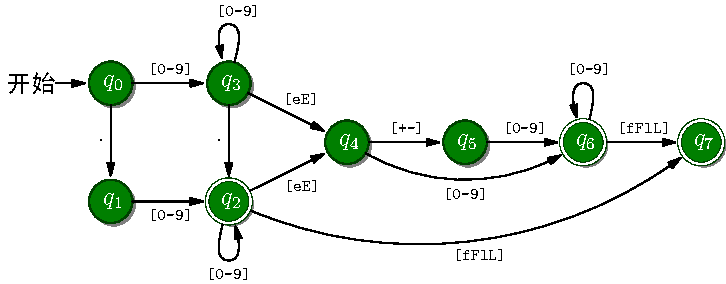
\includegraphics{automata.pdf}
  \caption{最终完成的有限自动机,同\autoref{fig:automata}}
  \label{fig:automatafinal}
\end{figure}

以上就是严教授画出\autoref{fig:automatafinal} 的全部代码。而且,更重要的是,
他为了画出这个有限自动机所做出的各种努力有着比画出这一幅图更多的回报:他可以
继续使用已经完成的 \prgname{simplenode} 模块方便地画出类似的自动机图形,并且
可以扩充这个模块,以完成更丰富的功能。

\section{习题和评注}

\begin{enumerate}
  \item 使用 \Asy{} 本身的 |object| 标签及连线机制,画出下面的状态转移图:
\begin{figure}[H]
  \centering
\begin{asy}
unitsize(2cm);
real margin = 2mm;
currentpen += 0.6;
object  q1 = draw("1", ellipse, (0,0), margin, FillDraw(lightblue)),
        q2 = draw("2", ellipse, (-1,-1), margin, FillDraw(lightblue)),
        q3 = draw("3", ellipse, (1,-1), margin, FillDraw(lightblue));
add(new void(picture pic, transform t) {
    draw(pic, "$\frac14$", point(q1,SW,t) -- point(q2,NE,t), Arrow);
    draw(pic, Label("$\frac34$",LeftSide), point(q1,SE,t) -- point(q3,NW,t),
         Arrow);
    draw(pic, "$\frac12$", point(q2,E,t) -- point(q3,W,t), Arrow);
    draw(pic, "$\frac12$", point(q2,WNW,t){WNW} .. point(q2,W,t)+t*W/4
         .. {-WSW}point(q2,WSW,t), ArcArrow);
    draw(pic, "$1$", point(q3,ESE,t){ESE} .. point(q3,E,t)+t*E/4
         .. {-ENE}point(q3,ENE,t), ArcArrow);
});
\end{asy}
\end{figure}
    注意其中自环箭头的绘制。

    利用 \prgname{simplenode} 重画此图,比较两种方式有什么不同。

  \item (此题较难)查看 \Asy{} 标准模块 \prgname{plain\_filldraw.asy} 中对
    |filltype| 类型的实现,参考 \cite{asyman} 的说明,分析其机制。在 \Asy{}
    1.91 中, |filltype| 被定义为:
\begin{asycode}[numbers=left]
struct filltype 
{
  typedef void fill2(frame f, path[] g, pen fillpen);
  fill2 fill2;
  pen fillpen;
  pen drawpen;

  int type;
  static int Fill=1;
  static int FillDraw=2;
  static int Draw=3;
  static int NoFill=4;
  static int UnFill=5;
      
  void operator init(int type=0, pen fillpen=nullpen, pen drawpen=nullpen,
                     fill2 fill2) {
    this.type=type;
    this.fillpen=fillpen;
    this.drawpen=drawpen;
    this.fill2=fill2;
  }
  void fill(frame f, path[] g, pen p) {fill2(f,g,p);}
}
\end{asycode}
    
    搞清楚:|fill2| 是什么类型?参考 |Fill| 等 |filltype| 填充类型的实现,尤
    其是其中 |RadialShade| 的实现,写一个 |Shadow| 的填充类型,完成前面严教授
    给结点画阴影函数相同的效果。在 \Asy{} 1.90 中 |RadialShade| 被实现为:
\begin{asycode}[numbers=left]
filltype RadialShade(pen penc, pen penr)
{
  return filltype(new void(frame f, path[] g, pen) {
    pair c=(min(g)+max(g))/2;
    radialshade(f,g,penc,c,0,penr,c,abs(max(g)-min(g))/2);
    });
}
\end{asycode}
    其效果是:
\begin{asycode}
object cat
    = draw("cat", ellipse, (0,0), xmargin=2mm, RadialShade(yellow, red));
\end{asycode}
\begin{figure}[H]
  \centering
\begin{asy}
object cat
    = draw("cat", ellipse, (0,0), xmargin=2mm, RadialShade(yellow, red));
\end{asy}
\end{figure}

  \item 仿照前面 |Circle| 函数的实现,为 \prgname{simplenode} 模块增加矩形、
    椭圆、菱形或是其他基本形状结点的构造函数,以便画出更丰富的图形。你可以需
    要一些额外的参数,如文字与边框的距离 |margin|。矩形结点的构造函数原型可以
    是这样的(你可以有不同的做法):
\begin{asycode}
node Rectangle(Label text, pair pos, pen textpen=currentpen,
               real margin=fontsize(textpen)/3, draw_t drawfn);
\end{asycode}
    应该能和 |Circle| 一样方便地使用不同的形状,如:
\begin{asycode}
node cat = Circle("cat", (0,0), filldrawer(yellow)),
     dog = Rectangle("dog", (3cm,0), filler(olive));
draw(cat, dog);
draw(cat .. bendleft .. dog, Arrow);
draw(dog .. bendleft .. cat, Arrow);
\end{asycode}
\begin{figure}[H]
  \centering
\begin{asy}
import "figure-src/simplenode.asy" as simplenode;

node Rectangle(Label text, pair pos, pen textpen=currentpen,
               real margin=fontsize(textpen)/3, draw_t drawfn)
{
    node nd;
    nd.pos = pos;
    label(nd.stuff, text, textpen);
    pair M = max(nd.stuff), m = min(nd.stuff);
    nd.outline = box(m-(margin,margin),M+(margin,margin));
    drawfn(nd.stuff, nd.outline);
    nd.E = nd.dir(E);
    nd.N = nd.dir(N);
    nd.W = nd.dir(W);
    nd.S = nd.dir(S);
    return nd;
}

node cat = Circle("cat", (0,0), filldrawer(yellow)),
     dog = Rectangle("dog", (3cm,0), filler(olive));
draw(cat, dog);
draw(cat .. bendleft .. dog, Arrow);
draw(dog .. bendleft .. cat, Arrow);
\end{asy}
\end{figure}

  \item 模仿 |bendleft|、|bendright| 的定义,为 \prgname{simplenode} 模块扩充
    |edgeconnector| 类型的连线方式。例如,可以增加水平、垂直方向的折线连接
    |HV|,它的用法类似于:
\begin{asycode}
node cat = Circle("cat", (0,0), filldrawer(yellow)),
     dog = Circle("dog", (4cm,3cm), filler(olive));
draw(cat, dog);
draw(cat .. HV .. dog, Arrow);
\end{asycode}
    \begin{figure}[H]
      \centering
\begin{asy}
import "figure-src/simplenode.asy" as simplenode;

path HV(node nd1, node nd2)
{
    path g1 = shift(nd1.pos) * nd1.outline;
    path g2 = shift(nd2.pos) * nd2.outline;
    pair c1 = (max(g1)+min(g1)) / 2;
    pair c2 = (max(g2)+min(g2)) / 2;
    pair z = (c2.x, c1.y);
    path edge = c1 -- z -- c2;
    edge = firstcut(edge, g1).after;
    edge = lastcut(edge, g2).before;
    return edge;
}

node cat = Circle("cat", (0,0), filldrawer(yellow)),
     dog = Circle("dog", (4cm,3cm), filler(olive));
draw(cat, dog);
draw(cat .. HV .. dog, Arrow);
\end{asy}
    \end{figure}
    再定义类似的 |VH|,它先画垂直的线,再画水平的线。(提示:|HV| 和 |VH| 的
    定义可能与 |operator--| 非常相似。)

  \item 在前面实现 |cat .. bendleft .. dog| 这种语法时,严教授使用一个函数作
    为中间类型。事实上也可以使用一个结构体。请补全下面的代码:
\begin{asycode}
typedef path edgeconnector(node nd1, node nd2);

// `\color{comment}中间类型`
struct node_con {
    node nd;
    edgeconnector con;
}

// `\color{comment}nd1 .. con .. nd2 的前一半`
node_con operator..(node nd, edgeconnector con)
{
    // ...
}

// `\color{comment}nd1 .. con .. nd2 的后一半`
path operator..(node_con nc, node nd)
{
    // ...
}
\end{asycode}

  \item 研究记法。
    \begin{enumerate}
      \item 在把多个 |draw_t| 类型的函数复合为一个函数时,严宇教授定义了
        |compose| 函数。但还可以进一步赋予函数复合一种新的记法,如使用加法运
        算符表示复合。试补全下面的实现:
\begin{asycode}
draw_t operator+(draw_t f1, draw_t f2)
{
    // ...
}
\end{asycode}
        并动手试验,能否把加法运算符函数的原型定义这个样子:
\begingroup
\renewcommand\thelstnumber{?}
\begin{asycode}[numbers=left]
draw_t operator+(... draw_t[] fns);
\end{asycode}
\endgroup
        并说明事实上前面定义的二元运算就已经足够了。

      \item 新记法的创立需要符合直观性。前面用加法运算符表示函数的复合函数的
        方式是否符合直观?把加法换成乘法怎么样?

      \item 严教授定义的 |shorten| 函数之所以能方便地使用,一个前提条件是在
        \Asy{} 中 |@| 运算符的优先级比 |--| 和 |..| 要低,因而在变换路径时不
        需要加括号。查阅资料或推测,\Asy{} 中不同运算符的优先级。设计实验并动
        手在 \Asy{} 环境中验证。并考虑在 \Asy{} 中所有可重载的运算符中,各自
        有什么语法特点或限制(能带几个参数、参数类型有没有限制等)。
    \end{enumerate}% 研究记法习题

  \item 严教授已经给出了几种 |draw_t| 的类型:|none|、|drawer|、|filler|、
    |filldrawer|、|shadow| 等等。请扩充 \prgname{simplenode} 中的定义,增加类
    似放射渐变填充类型 |RadialShade| 的效果。想想还有什么可以扩充的,比如说,
    \autoref{sec:object} 中球形立体效果的图形。

  \item\label{ex:flowchart} \Asy{} 的 \prgname{flowchart} 是用来画流程图的一
    个模块。它定义了一种特殊的记法,看起来很像严教授 \prgname{simplenode} 模
    块的用法,也有 \autoref{sec:object} 中 |object| 连线的影子。

    \prgname{flowchart} 
\end{enumerate}

本章的有限自动机及其表示的正则语言,可参看 \cite{aho1974},C 语言词法的形式化
描述参看 \cite{harbison2002}。

在 \Asy{} 中绘制图论图形一直没有很完善的官方模块,以往多是采用
\autoref{sec:object} 一节 |object| 类型的机制绘制的。随 \Asy{} 安装的基本模块
\prgname{flowchart} 是一个专用于绘制流程图的模块,里面定义了 |block| 类型,及
包括矩形、菱形、圆形、圆角矩形、斜多边形(bevel)在内的多种预定义形状,在安装
目录下可以找到例子。1.90 版以前的 \prgname{flowchart} 因为没有采用像本章所采
用的方便的记法,使用的方法与 |object| 类型类似,所以很不方便;自 1.91 版以后
的 \prgname{flowchart} 模块开始支持相对方便的记法了,实现的方法与本章中介绍的
类似。习题~\ref{ex:flowchart} 给出了 \prgname{flowchart} 的相关例子。使用
\prgname{flowchart} 并不足以完成本章带有阴影等修饰和曲线连线的图形,但有可能
扩充这个模板完成类似的功能。

加拿大 Waterloo 大学的博士生 Hubert Chan 曾给出过一个图论模块的框架
\prgname{graphtheory2.asy}(在
\url{http://asymptote.sourceforge.net/links.html} 有介绍),也完成了类似的功
能,并与本章给出的 \prgname{simplenode} 模块有相似,都使用了一些新的记法。

本章的 \prgname{simplenode} 模块是在作者在以前写的一个 \prgname{node} 模块的基
础上简化改编得到的,源代码可以在 \url{http://asy4cn.googlecode.com/} 找到。

本章中 \prgname{simplenode} 的一些设计受 \prgname{Ti\textit{k}Z} 宏包的影响,
参看 \cite{pgfman}。


\endinput

% vim:tw=77:

